\documentclass[beamer=true]{standalone}
\usepackage{../../preamblesnotes}

%Information to be included in the title page:
\title{第四課}
\author{功、能量和功率Work, energy and power}
\institute{周末班}
\date{}

\begin{document}
\frame{\titlepage}


\begin{frame}{能量Energy}
    \begin{itemize}
        \item 物體作功的能力。\\Energy is the capacity of a body for doing work.
        \item 以不同形式儲存在不同物體。\\Can be stored in different forms in different bodies.
        \item 可以轉移:\\Energy can be transferred:
              \begin{itemize}
                  \item 由一種形式轉移到另一種形式。\\From one form to another form
                  \item 由一個物體轉到另一個物體。\\From one body to another body
              \end{itemize}
        \item 單位Unit : J (焦耳Joule)
    \end{itemize}
\end{frame}

\begin{frame}{機械能Mechanical energy}
    \begin{itemize}
        \item 動能Kinetic energy(KE)
        \item 因物體移動而具有的能量。\\Stored in a body due to its motion.
        \item 量值Magnitude:$\frac{1}{2}mv^2$
    \end{itemize}\bigskip
    {\par\centering
        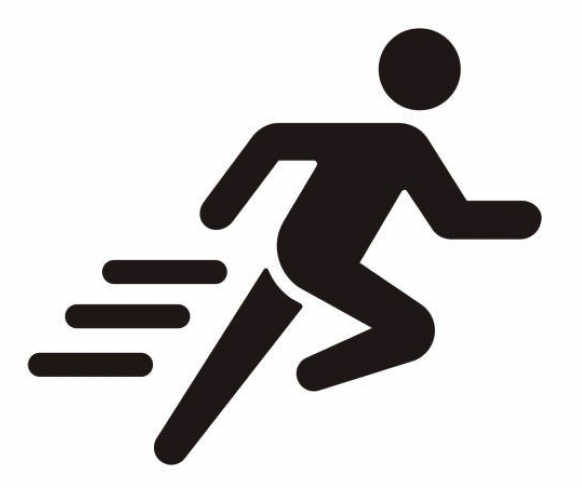
\includegraphics[width=.3\textwidth]{assets/8ff24777.png}
        \par}
\end{frame}

\begin{frame}{機械能Mechanical energy}
    \begin{itemize}
        \item 重力勢能Gravitational potential energy(GPE)
        \item 因物體離地面高度而具有的能量。\\Stored in a body due to its height.
        \item 量值Magnitude:$mgh$
    \end{itemize}\bigskip
    {\par\centering
        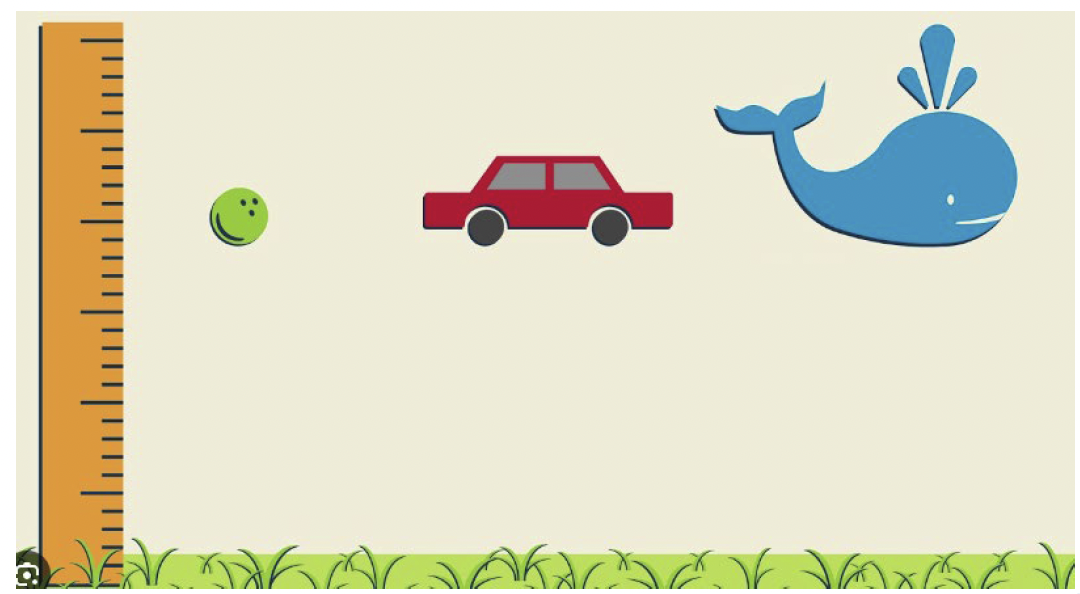
\includegraphics[width=.5\textwidth]{assets/86718add.png}
        \par}
\end{frame}

\begin{frame}{機械能Mechanical energy}
    \begin{itemize}
        \item 彈性勢能Elastic energy(EPE)
        \item 因物體形狀改變而具有的能量。\\Stored in a body due to its change of shape.
        \item EPE $\approx$ (改變程度 Change of shape)$^2$
    \end{itemize}\bigskip
    {\par\centering
        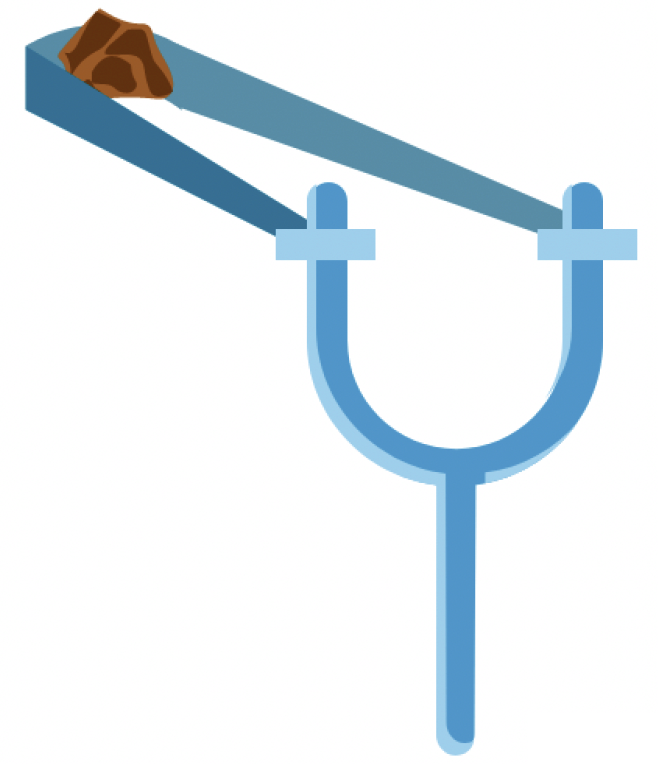
\includegraphics[width=.3\textwidth]{assets/aa983381.png}
        \par}
\end{frame}

\begin{frame}{非機械能Non-mechanical energy}
    例子Examples:
    \begin{itemize}
        \setlength{\itemsep}{12pt}
        \item 內能 Internal energy
        \item 化學能 Chemical energy
        \item 電勢能 Electrical energy
    \end{itemize}
\end{frame}


\begin{frame}{作功Work done}
    \begin{itemize}
        \item 力可以造成能量轉移,此時轉移的能量稱為機械功,或簡稱功。 \\Force transfer energy, the energy transferred is known as mechanical work, or work, for short.
        \item 作功是通過\textbf{施加力}使物體發生位移,而轉移能量的過程。\\Doing work is a process of energy transfer due to \textbf{applied force}.
        \item \fbox{$W=F\cdot s$}
    \end{itemize}
\end{frame}

\begin{frame}{作功Work done}
    \begin{itemize}
        \item 若力和位移不一定沿同一直線,作功的計算方式如下︰\\If the force and displacement are not necessarily along the same straight line, then the work done is calculated as follows:
    \end{itemize}
    \begin{alertblock}
        {作功Work done W}
        \begin{equation}
            W=F_\parallel \, s= F\, s\, \cos \theta
        \end{equation}
    \end{alertblock}
    {\par\centering
    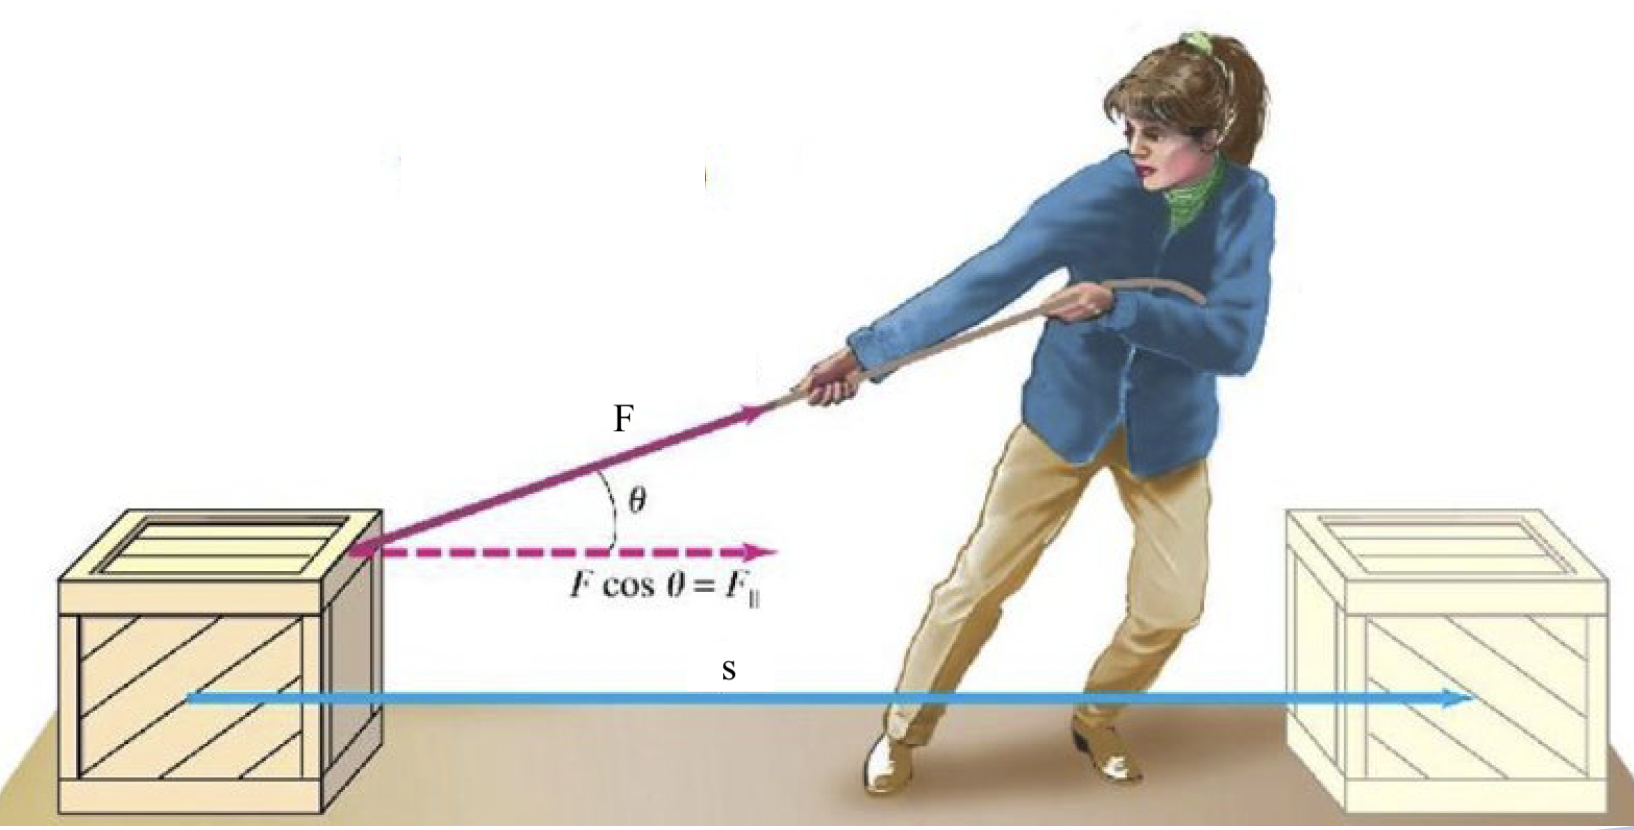
\includegraphics[width=.65\textwidth]{assets/af6c9fc3.png}
    \par}
\end{frame}
\begin{frame}{作功Work done}
    \begin{itemize}
        \item 做功的條件:\\Condition of doing work:
              \begin{itemize}
                  \item 存在施力(非淨力)\\Existance of applied force.
                  \item 施力使物件位移\\Applied force makes the object move.
                  \item 施力與位移不能垂直\\Applied force and displacement cannot be perpendicular.
              \end{itemize}
    \end{itemize}

\end{frame}

% \begin{frame}{功 Work}
%     功的特性:
%     標量
%     是一個能量轉移過程
% \end{frame}

\begin{frame}{功 Work}
    % \begin{columns}
    % \column{.5\textwidth}
    \begin{itemize}
        \item 重量的作功work done by weight=mgh
    \end{itemize}

    % \column{.5\textwidth}
    {\par\centering
    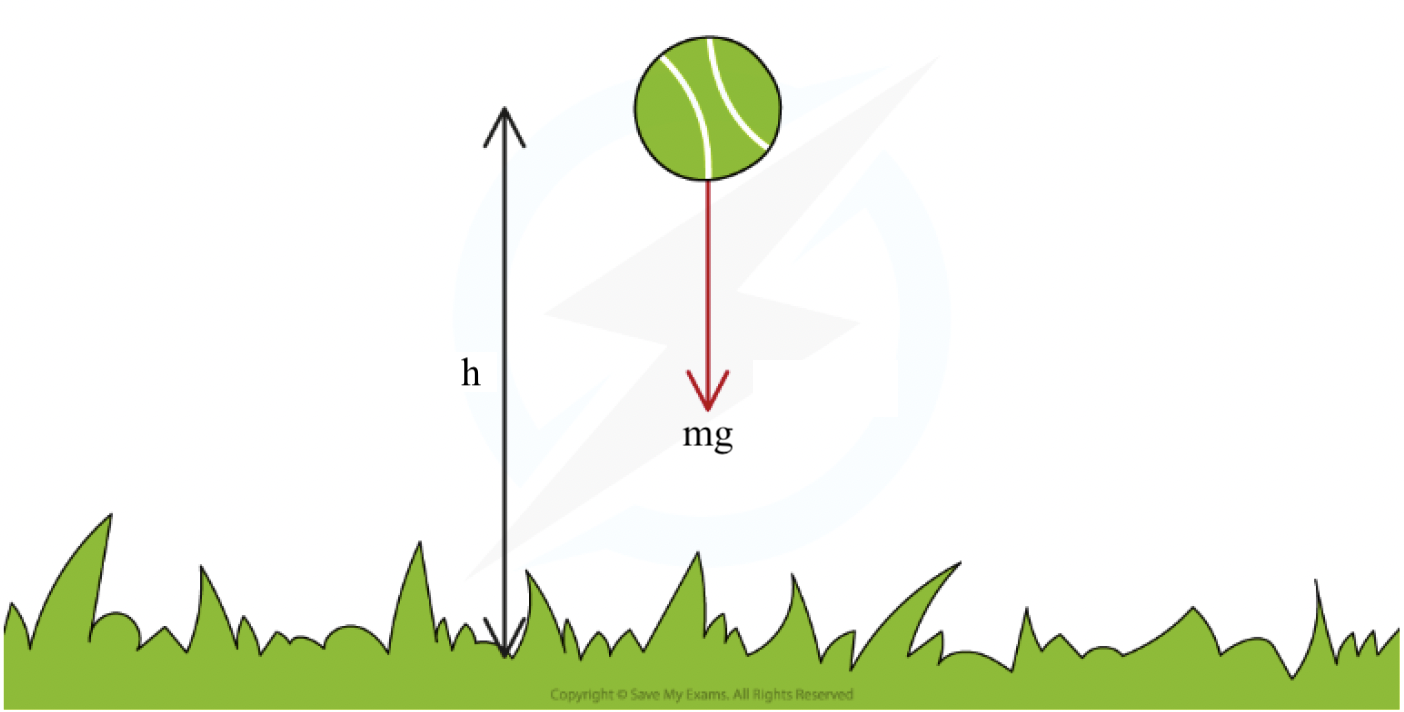
\includegraphics[width=.8\textwidth]{assets/55ada19f.png}
    \par}
    % \end{columns}
\end{frame}


\begin{frame}{功 Work}
    % \begin{columns}
    % \column{.5\textwidth}
    \begin{itemize}
        \item 阻力的作功\\work done by resistance = $-f\cdot s$
    \end{itemize}

    % \column{.5\textwidth}
    {\par\centering
    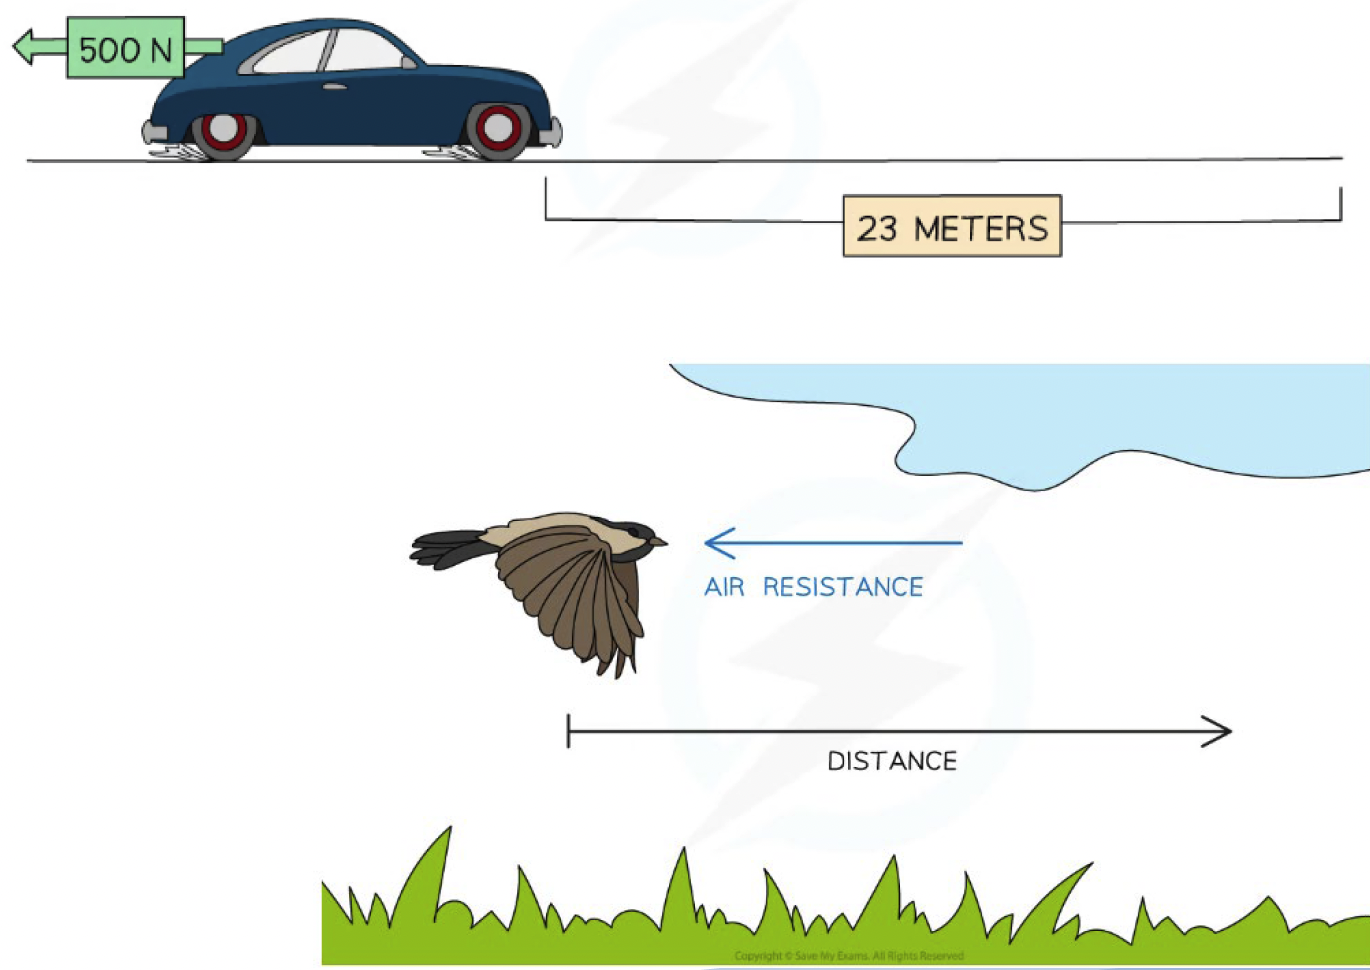
\includegraphics[width=.8\textwidth]{assets/f84b7953.png}
    \par}
    % \end{columns}
\end{frame}
\begin{frame}{功 Work}
    \begin{itemize}
        \item 人的施力的作功\\work done by applied force=0N
    \end{itemize}
    {\par\centering
    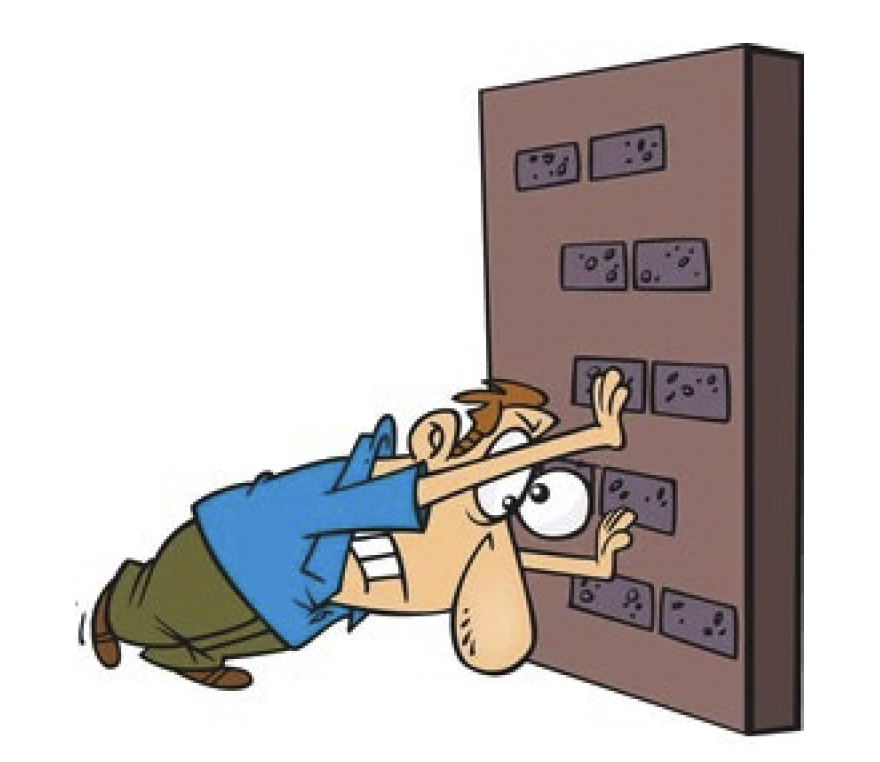
\includegraphics[width=.6\textwidth]{assets/5dba0df5.png}
    \par}
\end{frame}

\begin{frame}{功 Work}
    \begin{itemize}
        \item 施力方向垂直於位移\\Direction of applied force perpendicular to displacement
        \item[] 人對重物的作功\\Work done by applied force
        \item[] =0
    \end{itemize}
    {\par\centering
    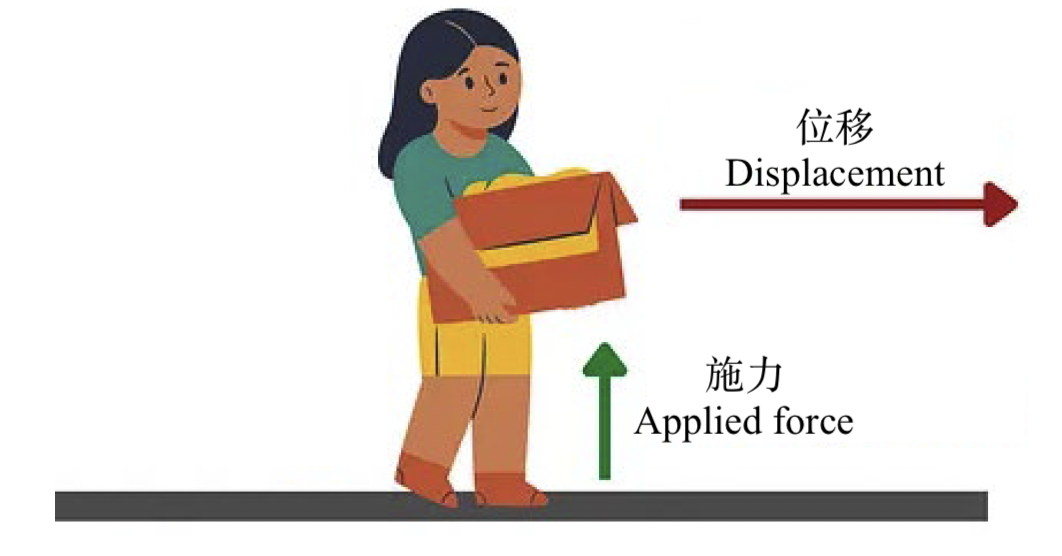
\includegraphics[width=0.66\textwidth]{assets/8303537c.png}
    \par}
\end{frame}

\begin{frame}{功 Work}
    \begin{itemize}
        \item 法向力垂直位移方向\\Normal reaction is perpendicular to displacement
        \item[] 冰地面的作功\\Work done by floor on snoopy
        \item[] =0
    \end{itemize}
    {\par\centering
    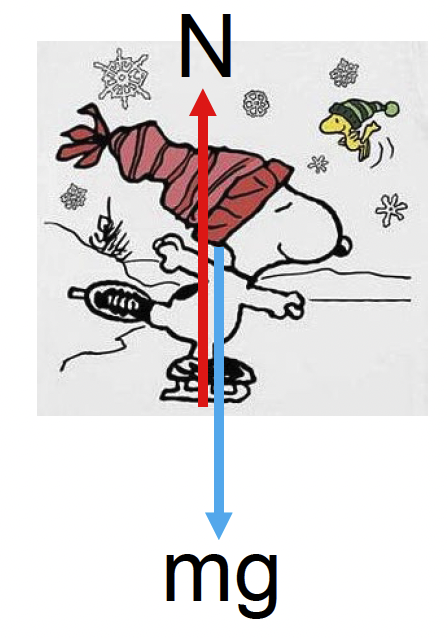
\includegraphics[width=.25\textwidth]{assets/330254f1.png}
    \par}
\end{frame}

\begin{eg}
    一個輕質金屬杯盛有水,水的初時溫度是 \oc{10}。這杯水在桌上滑行 16 cm 後停下,桌面與杯之間的摩擦力是 29 N。求水停下後的溫度。已知水的熱容量是 \hc{410}。 \\A light metal cup contains some water, the initial temperature of the water is \oc{10}. This cup of water slides on the table for 16 cm until it stops. The friction between table and cup is 29 N. Find the water temperature after the cup stops. Given that the specific heat capacity of the water is \hc{410}.
\end{eg}

\begin{eg}
    俯視圖繪出一堵光滑牆壁。一道力 F 如圖施加在一個小球上,使球沿牆壁滑動 3 m。球增加了 80 J 的能量。求 F 的量值。 \\The top-view diagram shows a smooth wall. A force F acts on the ball as shown, so that the ball slides against the wall for 3 m. The energy of the ball increases by 80 J. Find the magnitude of F.
        {\par\raggedleft
            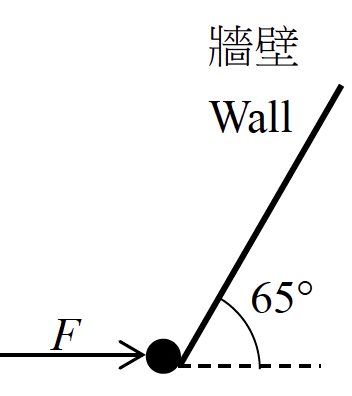
\includegraphics[width=.25\textwidth]{assets/f9626666.png}
            \par}
\end{eg}

\begin{eg}
    某人把行李箱傾斜\dg{25}以 45 N的力拉動,如圖所示。他把行李箱水平拉動了40 m。 \\A person pulls a luggage with 45 N force at a tilted angle of \dg{25}, as shown in the figure. He pulls the luggage for 40 m.
    \begin{itemize}
        \item[(a)] 求這人輸出的功。 \\Find the work done by the person.
    \end{itemize}
    \hfill{
        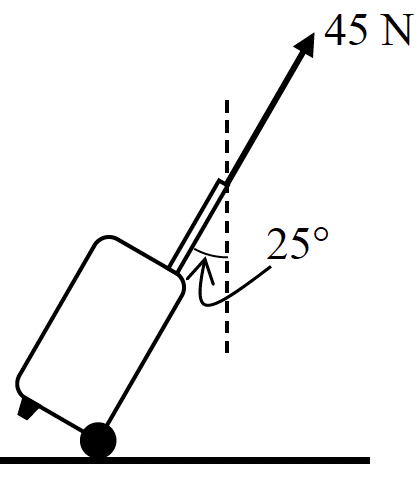
\includegraphics[width=.25\textwidth]{assets/1169635b.png}
        \par}
\end{eg}

\begin{eg}
    \begin{itemize}
        \item [(b)] 地面對行李箱的摩擦力是 15 N。 \\The friction between the ground and the luggage is 15 N.
              \begin{itemize}
                  \item [(i)]求這人克服摩擦力所作的功。\\ Find the work done by the person against friction.
              \end{itemize}
    \end{itemize}
\end{eg}

\begin{eg}
    \begin{itemize}
        \item [(b)] 地面對行李箱的摩擦力是 15 N。 \\The friction between the ground and the luggage is 15 N.
              \begin{itemize}
                  \item [(ii)] 為什麼 (a) 部的答案和 (b)(i) 的答案不相同?寫出一個可能原因。 \\Why do the answers in (a) and (b)(i) are not the same? State one possible reason.
              \end{itemize}
    \end{itemize}
\end{eg}

\begin{frame}{功 Work}
    \begin{exampleblock}
        {施力-位移關係圖  applied force - displacement graph}
        \begin{center}
            F的作功=F-s圖下的面積\\Work done by F = Area under F-s graph
        \end{center}
    \end{exampleblock}
    \bigskip
    {\par\centering
        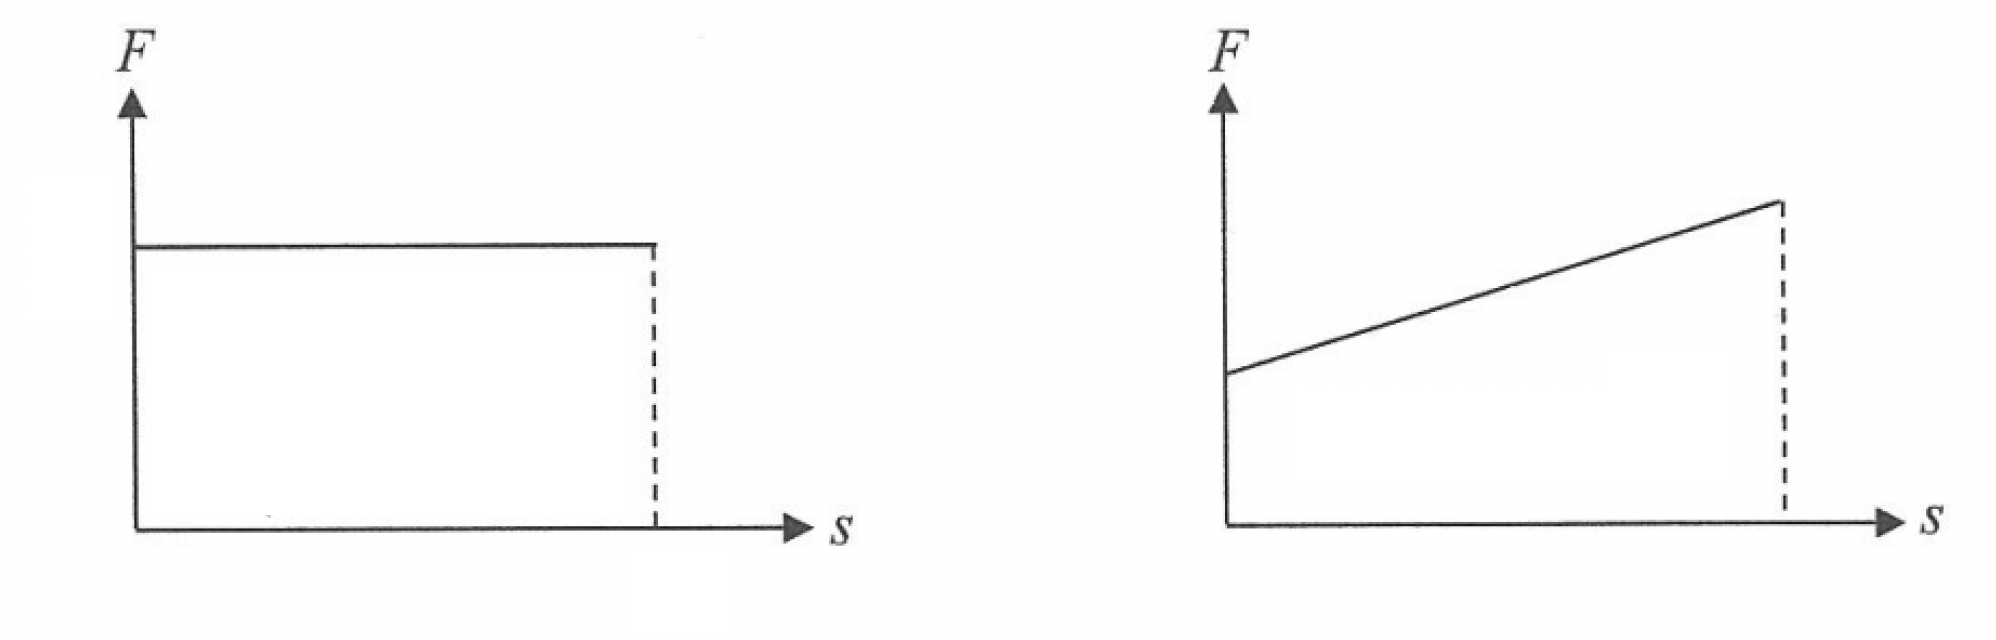
\includegraphics[width=.7\textwidth]{assets/f964c556.png}
        \par}
\end{frame}


\begin{frame}{動能Kinetic energy}
    \begin{itemize}
        \item 移動的物體具有動能(KE)。若物體的質量為 $m$,移動的速率為 $v$,則它的動能計算方式如下︰\\ A moving object possesses kinetic energy (K.E.). If the mass and the moving speed of the object are $m$ and $v$ respectively, then its kinetic energy can be calculated as follow:
    \end{itemize}
    \begin{alertblock}
        {動能Kinetic energy KE}
        \begin{equation}
            KE=\frac{1}{2}mv^2
        \end{equation}
    \end{alertblock}
    \begin{itemize}
        \item 動能改變:Change of kinetic energy:
              \begin{itemize}
                  \item 均速Uniform speed $\rightarrow$ 動能改變KE change  $=0$
                  \item 加速Acceleration($a>0$) $\rightarrow$ 動能增加KE gain $=\frac{1}{2}mv^2-\frac{1}{2}mu^2$
                  \item 減速Deceleration($a<0$) $\rightarrow$ 動能減少KE loss $=\frac{1}{2}mu^2-\frac{1}{2}mv^2$
              \end{itemize}
    \end{itemize}
\end{frame}


\begin{frame}{動能Kinetic energy}
    \par
    {\par\centering
        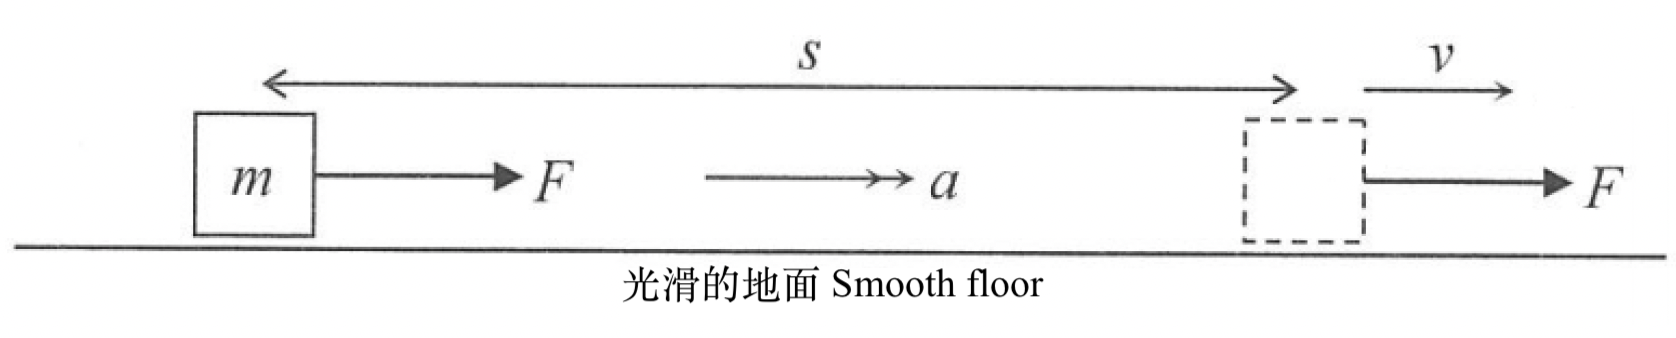
\includegraphics[width=0.66\textwidth]{assets/7304acb1.png}
        \par}
    \begin{itemize}
        \item[] $u=0$
        \item[] $v^2=2as$
        \item[] 作功Work done $=Fs=mas=\frac{1}{2}mv^2$
    \end{itemize}
\end{frame}

\begin{eg}
    圖中是一架車子的動能和時間的平方的情況。車的質量是5000kg。找出車的加速度。\\The graph shows the relationship between the kinetic energy and the square of time for a car. The mass of the car is 5000kg. Find the acceleration of the car.
        {\par\raggedleft
            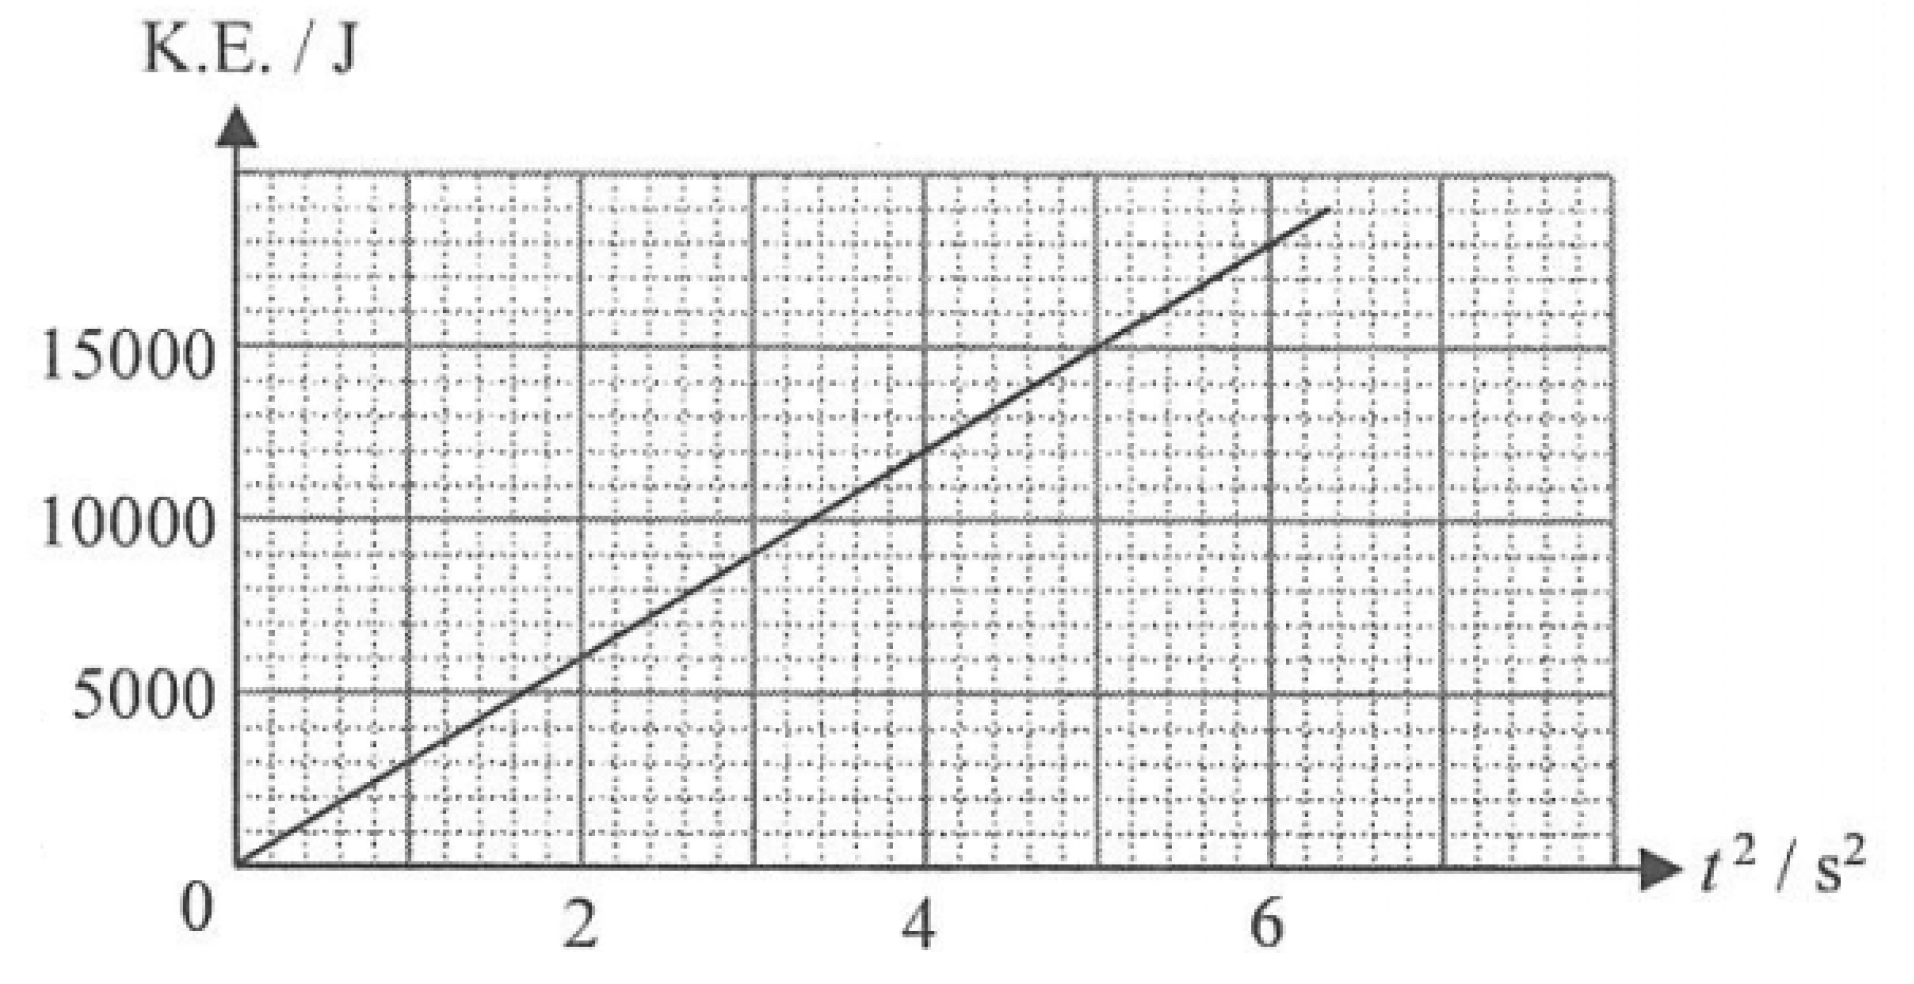
\includegraphics[width=0.6\textwidth]{assets/3643740d.png}
            \par}
\end{eg}

% \begin{frame}{重力勢能Gravitational potential energy}
%     \begin{itemize}
%         \item 重力勢能是物體在重力作用下所具有的能量,大小隨物體的位置而改變。\\Gravitational energy is the energy stored in an object under gravitational forces, and it changes as the position of the object changes.
%         \item 當物體移到較高的位置,它的重力勢能便會增加。\\If an object moves to a higher position, its gravitational potential energy increases.
%     \end{itemize}



% \end{frame}

\begin{frame}{重力勢能Gravitational potential energy}
    \begin{itemize}
        \item 假設質量為 $m$ 的物體受力 $F$($=mg$ ) 作用,以恆速度從地面上升至高度 $h$,$F$ 對物體作功,轉移到物體的能量成為它獲得的勢能(PE),勢能的計算公式如下︰\\If a force $F$($=mg$ ) acts on an object of mass $m$ so that it ascends for a height $h$, $F$ does work on the object and increases the potential energy of the object, it is calculated as follow:
    \end{itemize}
    \bigskip
    \begin{alertblock}
        {重力勢能Gravitational potential energy (GPE)}
        \begin{equation}
            GPE=mgh
        \end{equation}
    \end{alertblock}
\end{frame}

\begin{frame}{重力勢能Gravitational potential energy}
    \begin{columns}
        \column{0.6\textwidth}
        \begin{itemize}
            \item 把物件從地面(參考位置)到 $h$ 的高度所需的能量\\Required energy to move an object from ground(reference point) to height of $h$
            \item = 施力$F$ 到$h$ 所作的功 \\=Work done by applied force $F$ to move it to $h$
            \item[*] 假設地球重量不會隨$h$ 改變(重力場固定)\\Assuming that gravity does not change with h (gravitaional field strength remains constant)
        \end{itemize}
        \column{0.4\textwidth}
        {\par\centering
            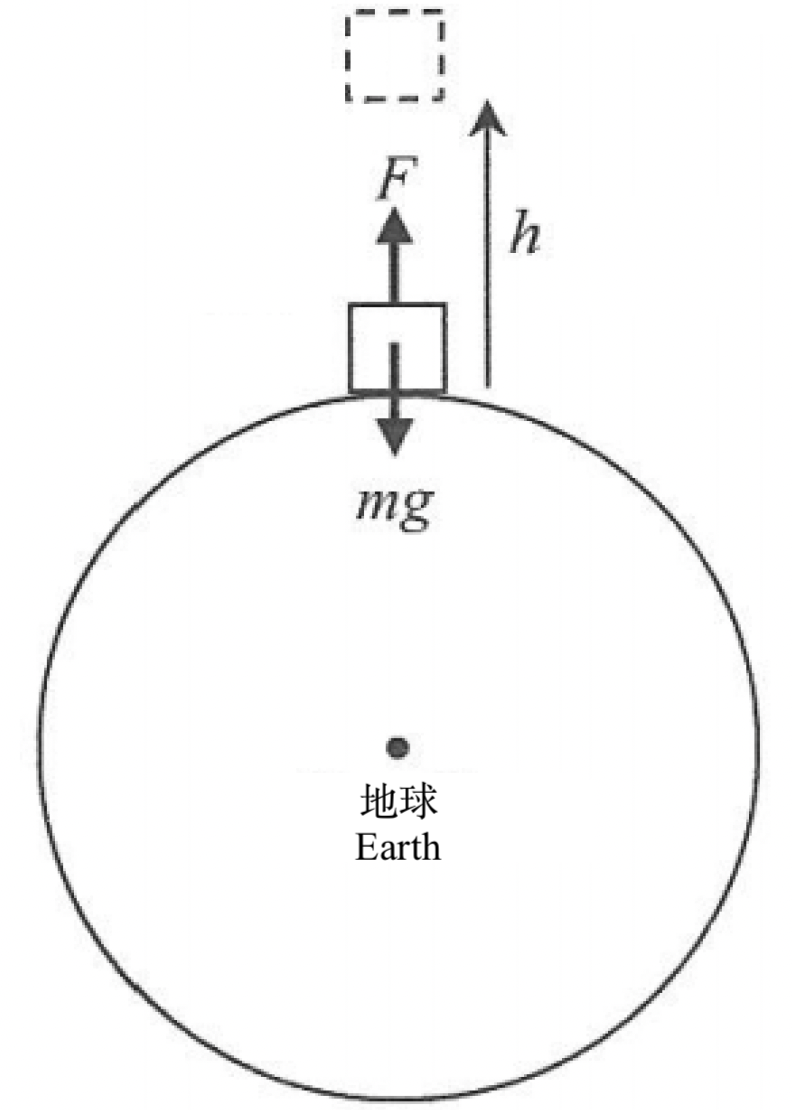
\includegraphics[width=.8\textwidth]{assets/9272e1df.png}
            \par}
    \end{columns}
\end{frame}

\begin{frame}{重力勢能改變Change of gravitational potential energy}\par
    {\par\centering
        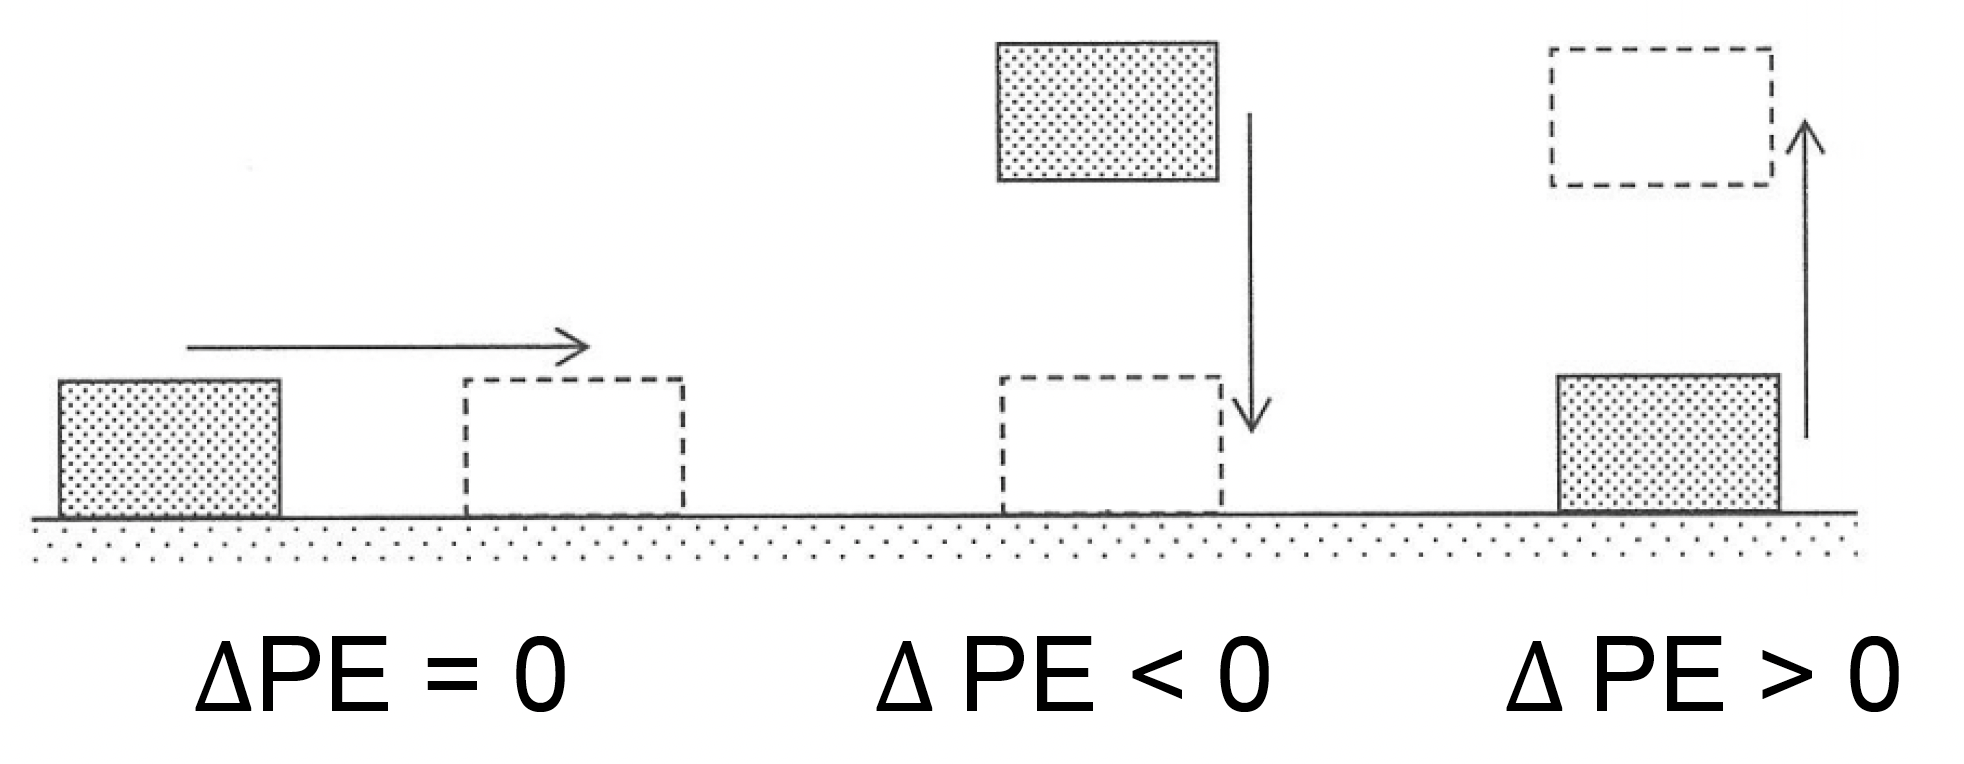
\includegraphics[width=.8\textwidth]{assets/0a3fcefd.png}
        \par}
\end{frame}

\begin{frame}{彈性勢能Elastic potential energy}
    \begin{columns}
        \column{0.5\textwidth}
        \begin{itemize}
            \setlength{\itemsep}{15pt}
            \item 當彈簧被\textbf{壓縮}或\textbf{伸展},EPE儲存在彈簧中。 $\rightarrow$ EPE $>0$\\When spring is \textbf{compressed} or \textbf{stretched}, EPE is stored in the spring. $\rightarrow$ EPE $>0$
            \item 當彈簧回到\textbf{原來長度}時,EPE會被釋放。 $\rightarrow$ EPE $=0$\\When spring is put to its \textbf{natural length}, EPE is released. $\rightarrow$ EPE $=0$
            \item EPE $=\dfrac{1}{2}k\, x^2$ (out-syl)
        \end{itemize}
        \column{0.5\textwidth}
        {\par\centering
            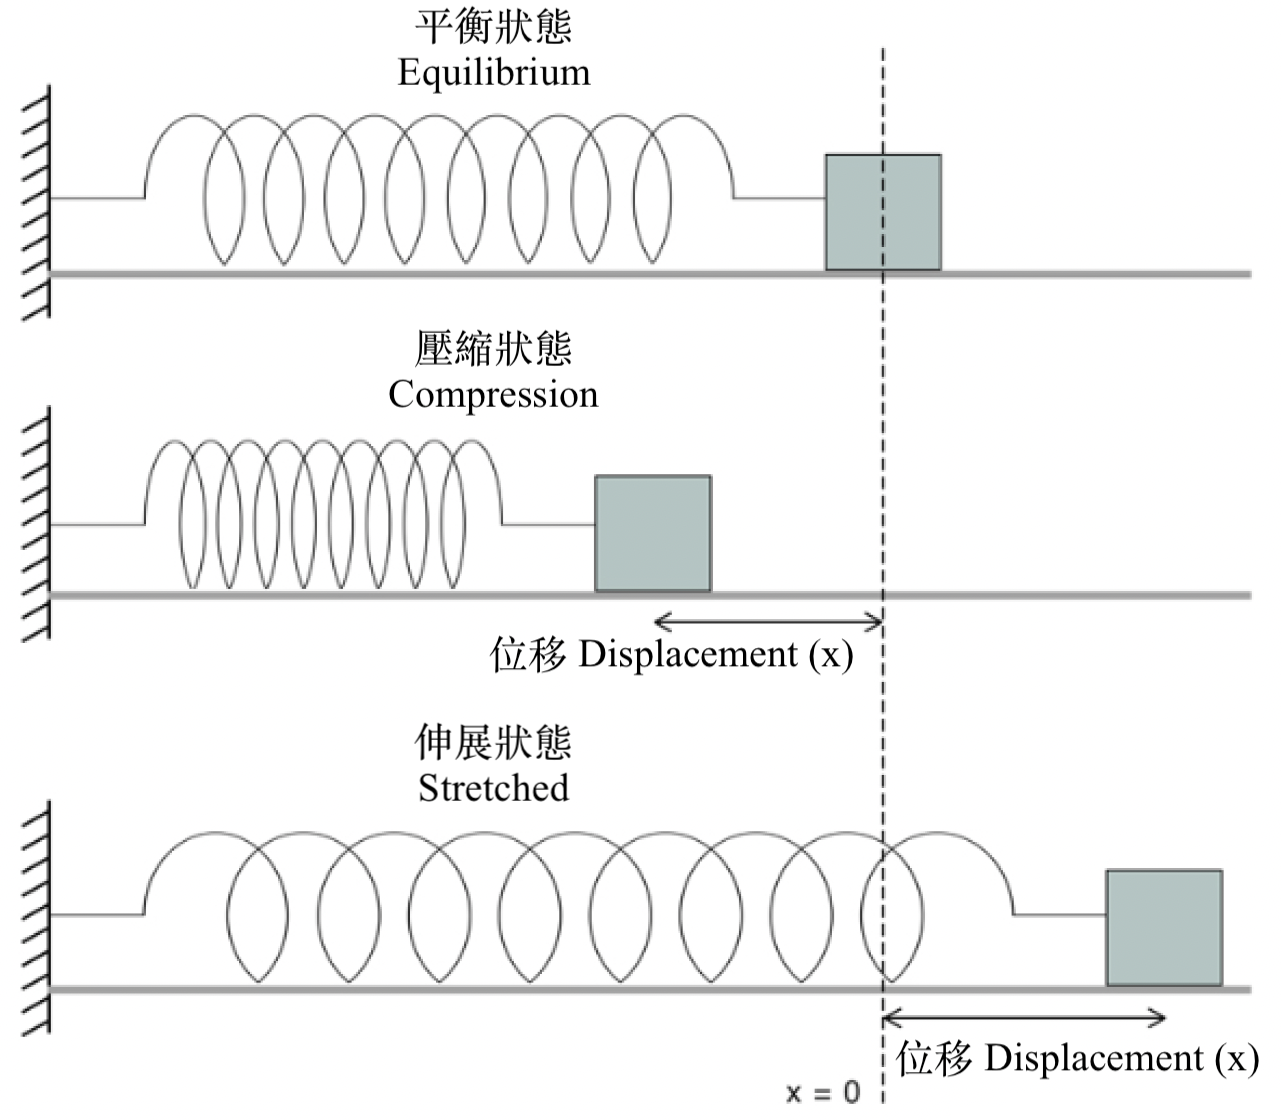
\includegraphics[width=\textwidth]{assets/5c1cf9fc.png}
            \par}
    \end{columns}
\end{frame}

\begin{frame}{彈性勢能Elastic potential energy}
    \begin{columns}
        \column{0.5\textwidth}
        \begin{itemize}
            \setlength{\itemsep}{12pt}
            \item F-s圖面積\\Area under F-s graph
            \item []=從平衡位置到s的作功\\=Work done from equilibrium position to s
            \item []=儲存的彈性勢能\\=EPE stored
        \end{itemize}\bigskip
        {\par\centering
            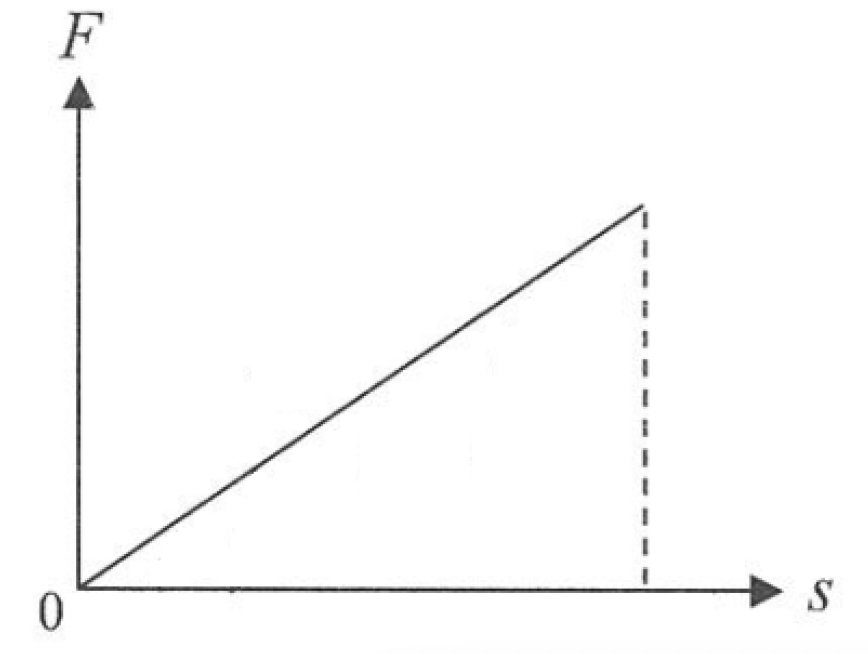
\includegraphics[width=0.66\textwidth]{assets/80e4b012.png}
            \par}
        \column{0.5\textwidth}
        {\par\centering
            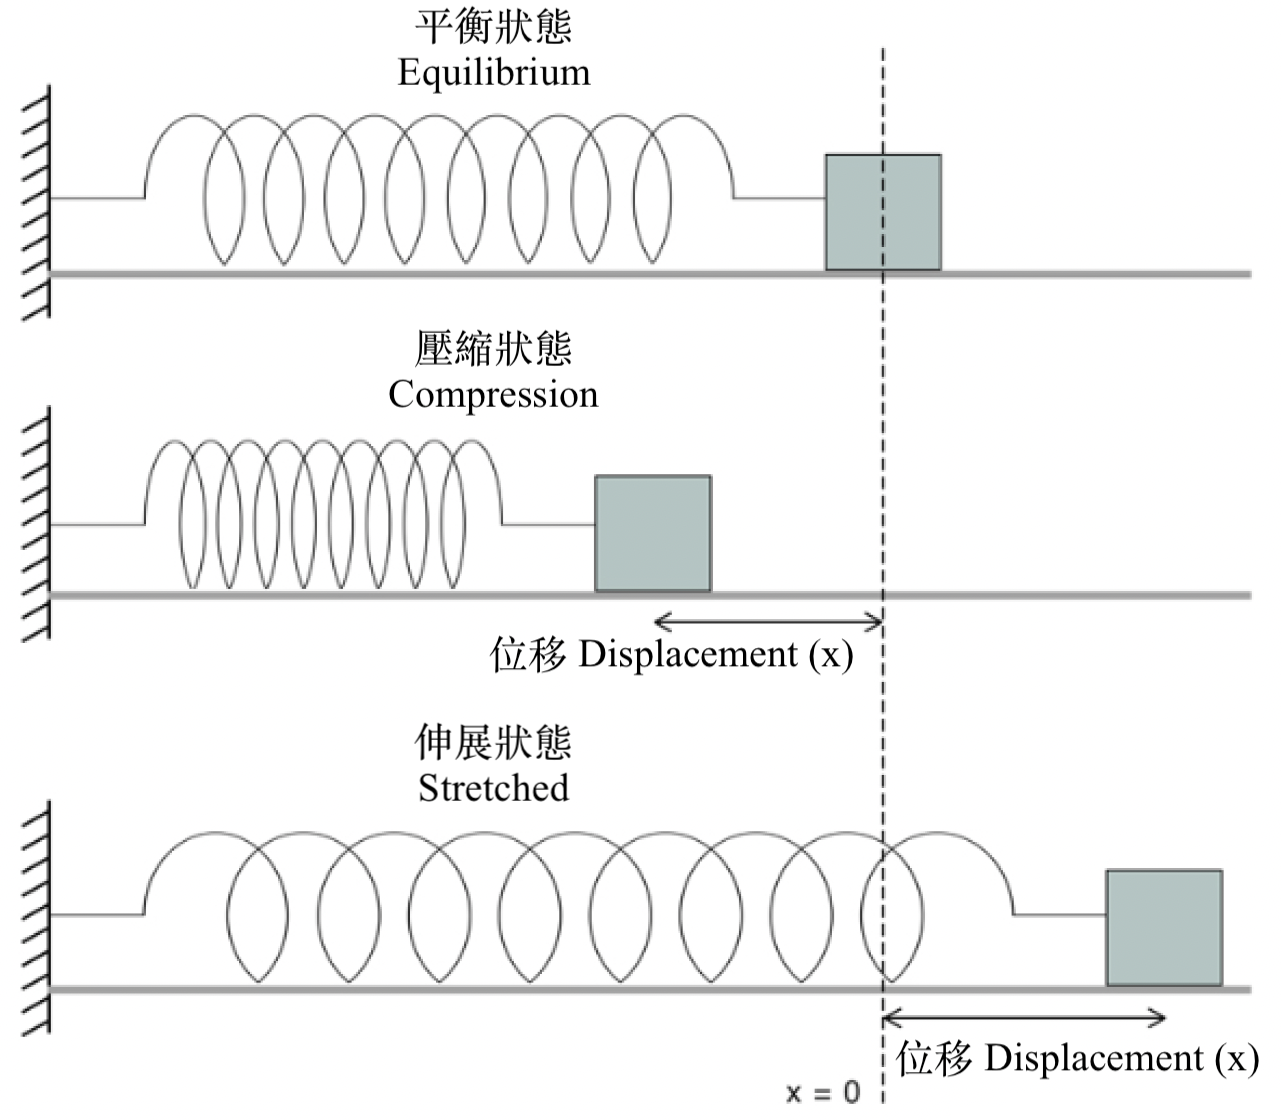
\includegraphics[width=\textwidth]{assets/5c1cf9fc.png}
            \par}
    \end{columns}
\end{frame}

\begin{frame}{能量守恆定律Conservation of energy}
    \begin{itemize}
        \item 能量守恆定律指出:能量可以從一種形式轉換為另一種形式,但能量既不可能創造出來,也不可能被毀滅。\\The law of conservation points out that: Energy can transform from one form to the other, but energy can neither be created nor destroyed.
              \begin{itemize}
                  \item 一個獨立系統的總能量=固定不變\\Total energy in an isolated system = constant.
              \end{itemize}
    \end{itemize}
\end{frame}

\begin{frame}{能量守恆定律Conservation of energy}
    \begin{itemize}
        \item 假如沒有作功,總機械能必須守恆。\\If there is no work done on the sysyem, the total mechanical energy must be conserved.
    \end{itemize}
    \begin{exampleblock}
        {機械能守恆Conservation of mechanical energy}
        \begin{align*}
            \textrm{總機械能Total mechanical energy} & =KE+GPE+EPE          \\
                                                 & =\textrm{常數constant}
        \end{align*}
    \end{exampleblock}
    \begin{itemize}
        \item 假如沒有彈性物件,\\If there is no elastic object,
        \item[] \fbox{$KE+GPE=$ 常數constant}
    \end{itemize}
\end{frame}

\begin{eg}
    圖中顯示浩賢在遊樂場乘坐摩天輪的情況,若摩天輪勻速轉 動,浩賢的哪一項物理量保持不變?\\The figure shows the situation of Haohan riding a Ferris wheel at the park. If the Ferris wheel rotates at a constant speed, which physical quantity of Haohan remains unchanged?
    {\par\centering
    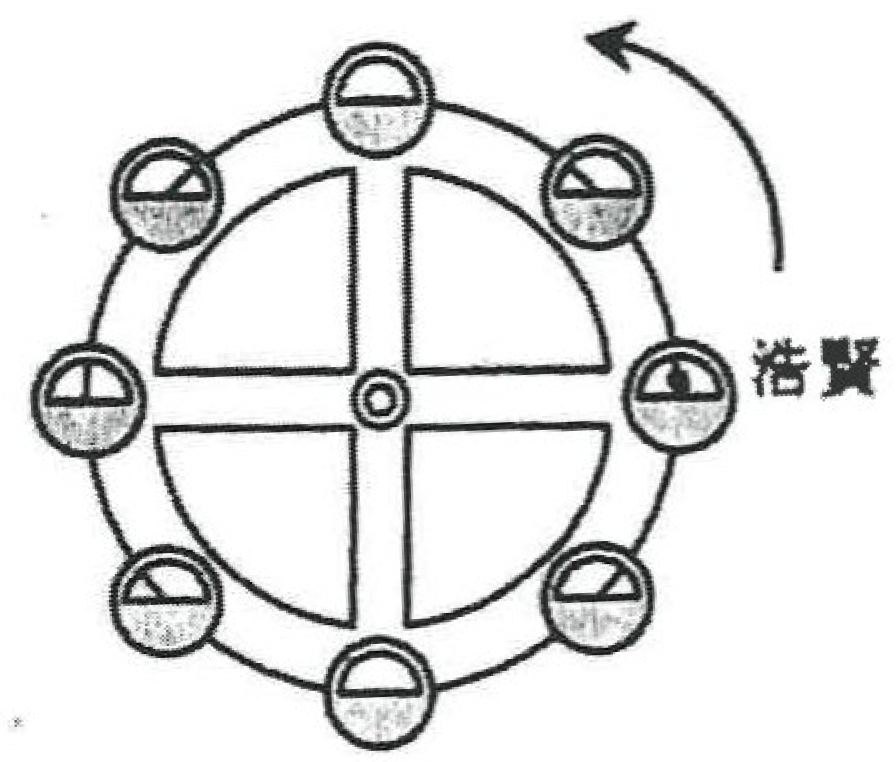
\includegraphics[width=0.25\textwidth]{assets/54a93bf1.png}
    \par}
    \begin{tasks}(2)
        \task 速度Velocity
        \task 動能Kinetic energy
        \task 勢能Potential energy
        \task 總機械能Total mechanical energy
    \end{tasks}
\end{eg}

\begin{eg}
    一個質量為 0.2 kg 的粒子在P點從靜止釋放,粒子沿軌道 PQR 滑行至R點。 \\A particle of mass 0.2 kg is released at P from rest, the particle slides to R alone PQR.
        {\par\centering
            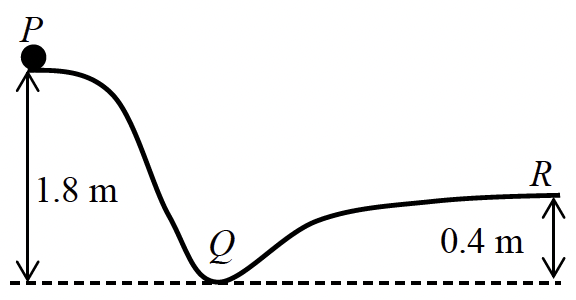
\includegraphics[width=.4\textwidth]{assets/047b1413.png}
            \par}

\end{eg}

\begin{eg}
    \begin{itemize}
        \item [(a)]取 Q 點的高度為零,求粒子在 P 點時的 重力勢能。 \\Set the height of Q be zero, find the potential energy of the particle at P.
    \end{itemize}{\par\raggedleft
    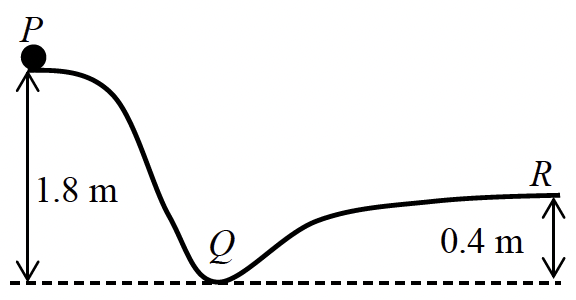
\includegraphics[width=.4\textwidth]{assets/047b1413.png}
    \par}
\end{eg}

\begin{eg}
    \begin{itemize}
        \item [(b)] 假設軌道PQR光滑。求粒子在 R 點時的速率。 \\Assume that the track PQR is smooth. Find the speed of the particle at R.
    \end{itemize}{\par\raggedleft
    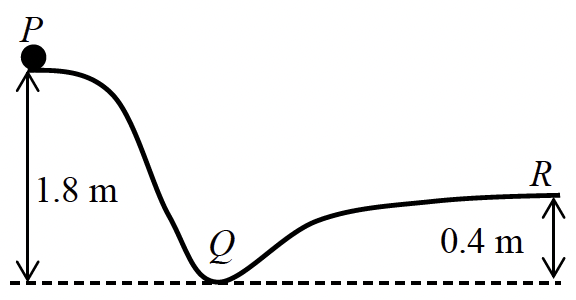
\includegraphics[width=.4\textwidth]{assets/047b1413.png}
    \par}
\end{eg}

\begin{eg}
    \begin{itemize}
        \item[(c)] 實際上,粒子到達R點時,速率只有 (b) 部答案的 75\%。若軌道 PQR 長 2 m, 求粒子滑行期間受到的平均摩擦力。 \\In fact, the speed of the particle arrives at R is 75\% of the answer in (b). If the length of the track PQR is 2 m, find the average friction of the particle as it slide on the track.
    \end{itemize}{\par\raggedleft
    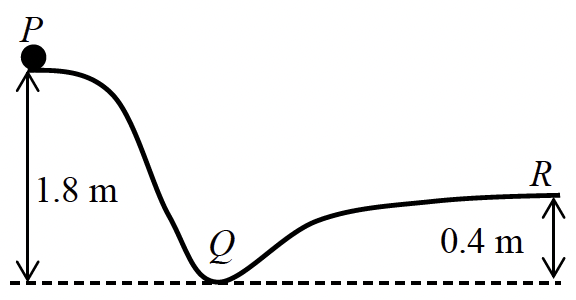
\includegraphics[width=.4\textwidth]{assets/047b1413.png}
    \par}
\end{eg}

\begin{eg}
    一個 5 kg 方塊如圖以滑輪懸掛在 1.3 m高處。繩子另一端是放在光滑水平桌面的 7 kg 方塊。現把系統從靜止釋放直至 5 kg 方塊撞擊地面。 \\A 5 kg block is hung at the height of 1.3 m. The other end of the string is a 7 kg block on a smooth horizontal table. The system is released from rest until the 5 kg block hits the ground.
        {\par\centering
            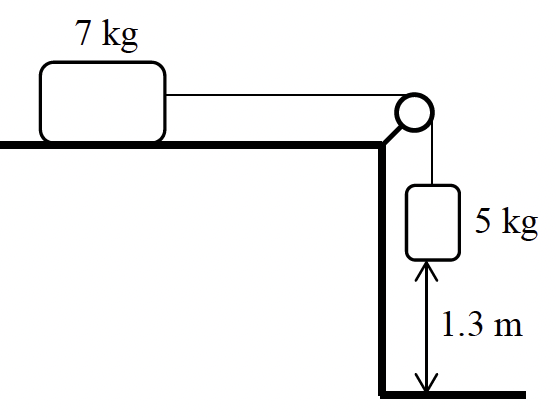
\includegraphics[width=.35\textwidth]{assets/8a2c64de.png}
            \par}
\end{eg}

\begin{eg}
    \begin{itemize}
        \item[(a)] 求 5 kg 方塊撞擊地面前損失的重力勢能。 \\Find the loss of GPE of the 5 kg block before it hits the ground.
    \end{itemize}
\end{eg}

\begin{eg}
    \begin{itemize}
        \item [(b)] 由此,求 5 kg 方塊撞擊地面一刻的速率。 Hence, find the speed of the 5 kg block at the moment when it hits the ground.
    \end{itemize}
\end{eg}

\begin{eg}
    某跳水運動員在水面上 5 m 處以 \vel{2} 的速率垂直跳起,並落在水面。忽略空氣阻力。 \\A diver jumps vertically upward at 5 m above the water surface at the speed \vel{2}, and then he enters the water. Ignore air resistance.
    \begin{itemize}
        \item [(a)] 求跳水運動員落在水面時的速率。 \\Find the speed of the diver as he arrives at the water surface.
    \end{itemize}
\end{eg}

\begin{eg}
    \begin{itemize}
        \item [(b)] 已知運動員的質量是 60 kg。若他最深能達到水面下2.4 m,求他在水中下降期 間,水對他施力的平均力量值。 \\Given that the mass of the diver is 60 kg. If he can arrive 2.4 m below the water surface at the deepest, find the magnitude of the average force acting on the diver as he descends in water.
    \end{itemize}
\end{eg}

\begin{eg}
    斜面上的點Y位於XZ的中間。兩個質量相同的粒子A和B分別從X和Y處靜止釋放。以下哪些關於A和B的陳述是正確的?\\Point Y on the incline is located in the middle of XZ. Two particles A and B, with equal masses, are released from rest at points X and Y, respectively. Which of the following statements about A and B are correct?\bigskip
    {\par\centering
        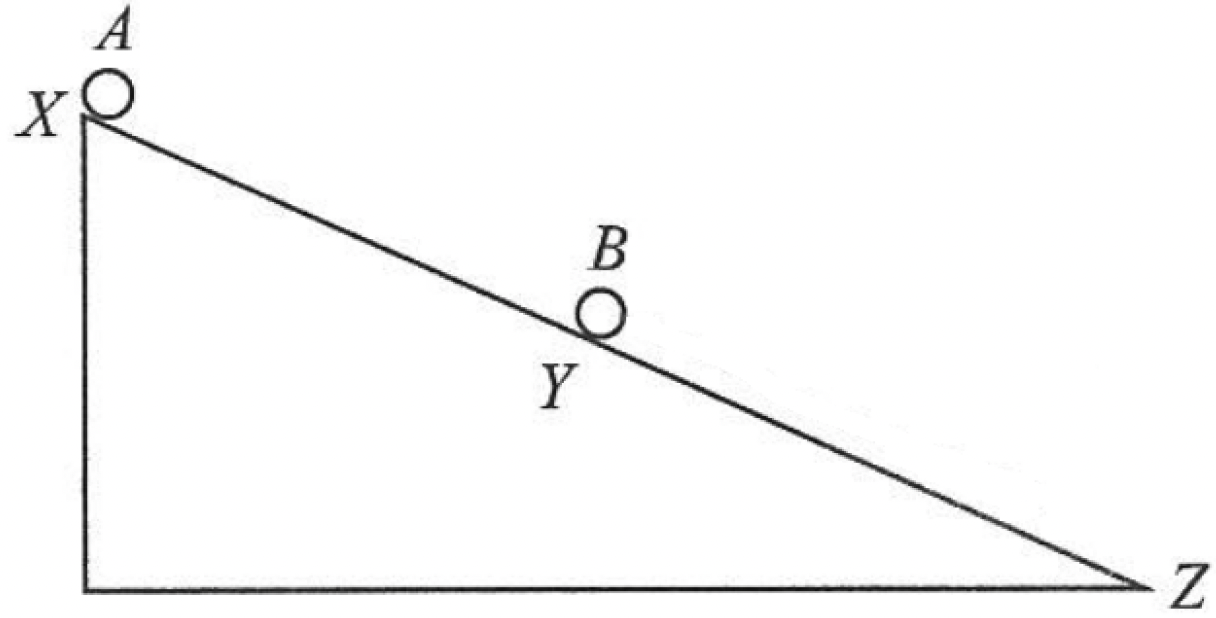
\includegraphics[width=0.45\textwidth]{assets/7f1967a5.png}
        \par}
\end{eg}
\begin{eg}

    \begin{statements}
        \task 粒子A在Z點的勢能是粒子B在Z點勢能的兩倍。\\The potential energy of particle A at point Z is twice that of particle B at point Z.
        \task 粒子A在Z點的動能是粒子B在Z點的動能的兩倍。\\The kinetic energy of particle A at point Z is twice that of particle B at point Z.
        \task 粒子A到達Z所需的時間是粒子B到達Z所需時間的兩倍。\\Time required for particle A to reach Z is twice as long as particle B to reach Z.
    \end{statements}
\end{eg}

\begin{frame}{單擺Simple pendulum}
    \par
    {\par\centering
        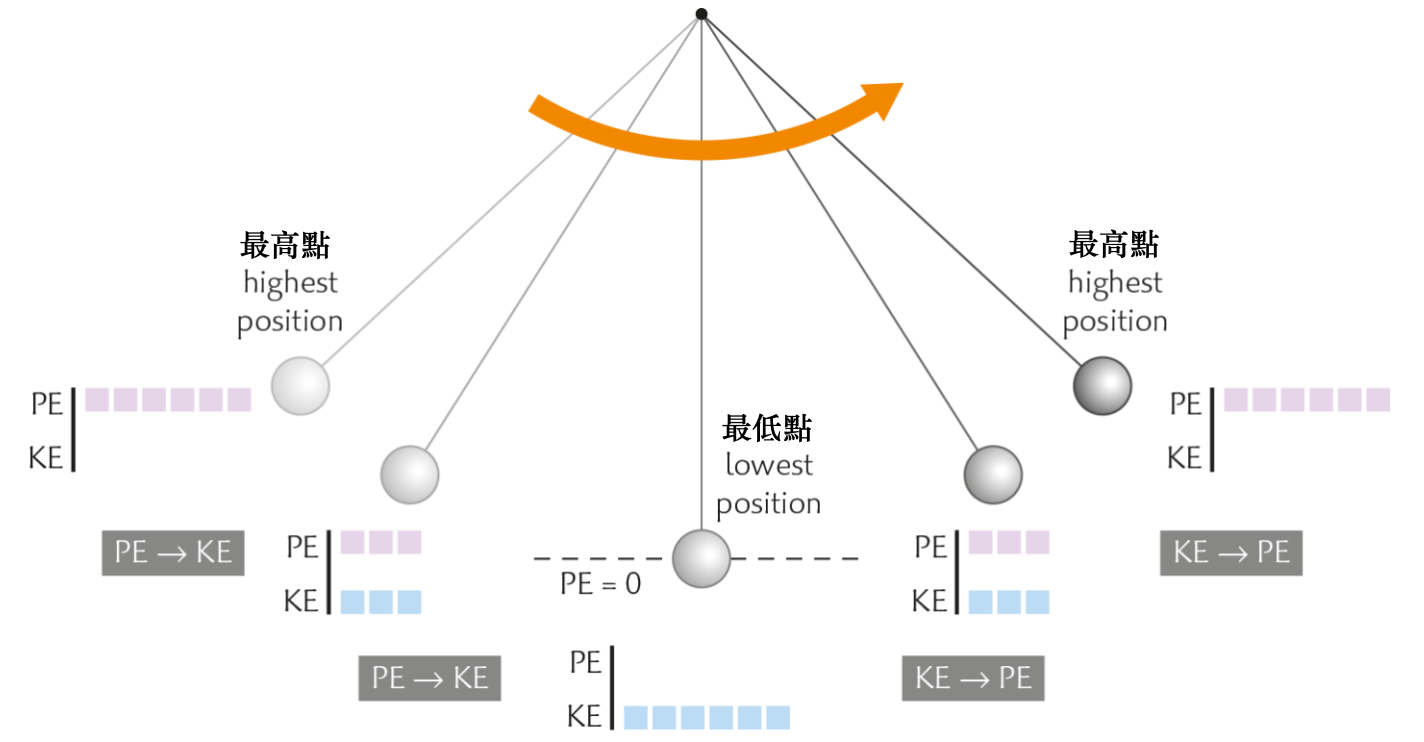
\includegraphics[width=\textwidth]{assets/76d2fb7c.png}
        \par}
\end{frame}

\begin{frame}{彈床Trampoline}
    \par
    {\par\centering
        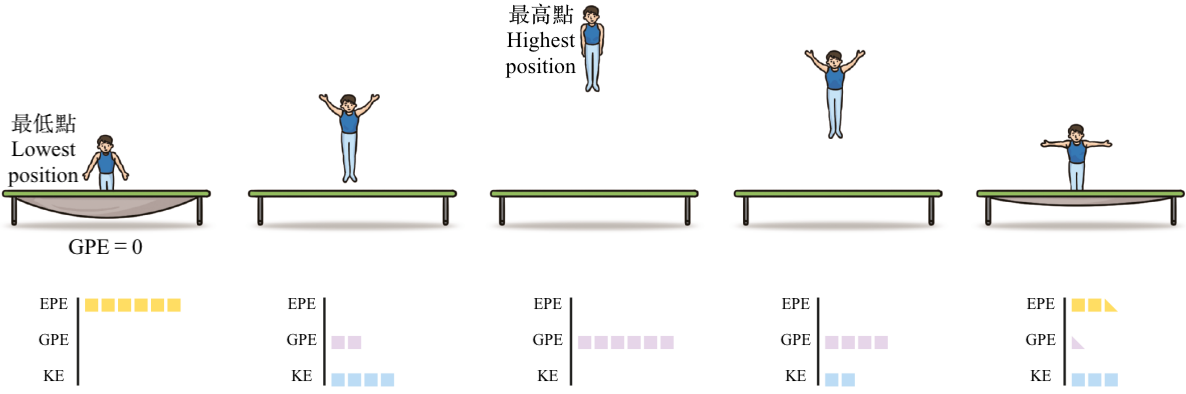
\includegraphics[width=\textwidth]{assets/eaf85404.png}
        \par}
\end{frame}

\begin{frame}{過山車Roller coaster}
    \par
    {\par\centering
        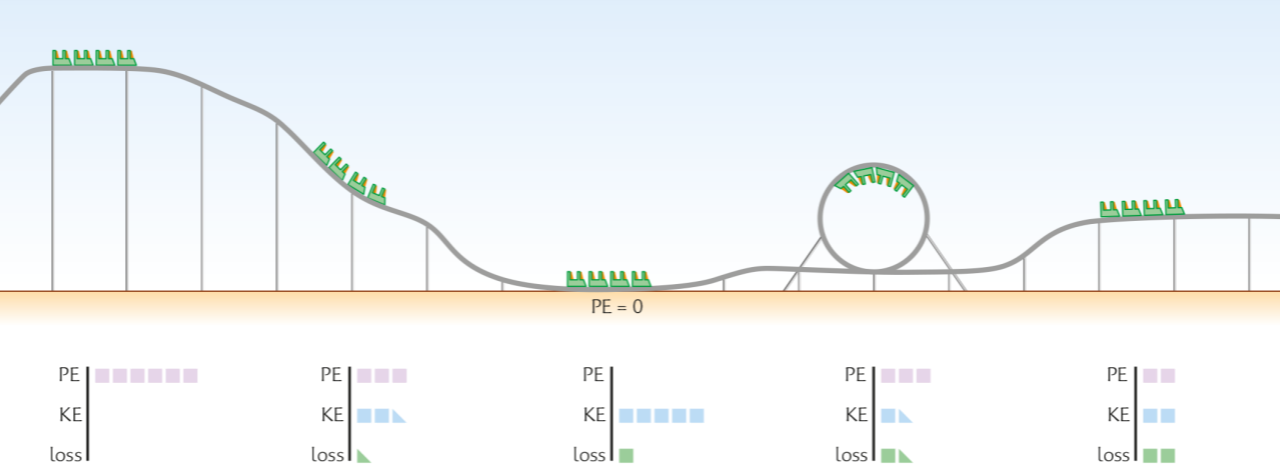
\includegraphics[width=\textwidth]{assets/d6c1ec53.png}
        \par}
\end{frame}

\begin{frame}{跳水High diving}
    \par
    {\par\centering
        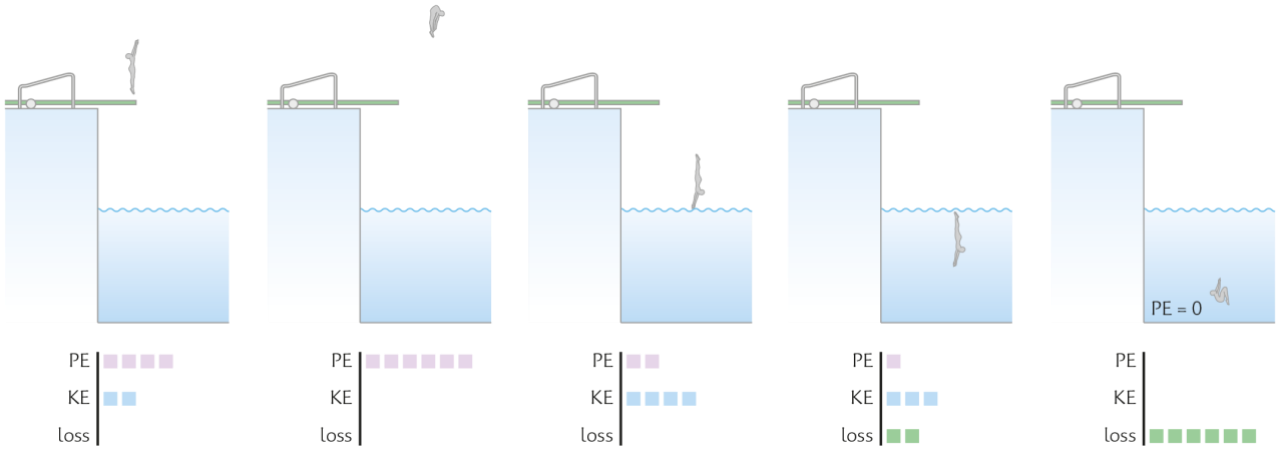
\includegraphics[width=\textwidth]{assets/b76432a0.png}
        \par}
\end{frame}

\begin{frame}{自由落體的圖Free fall graphs}
    \par{\par\centering
        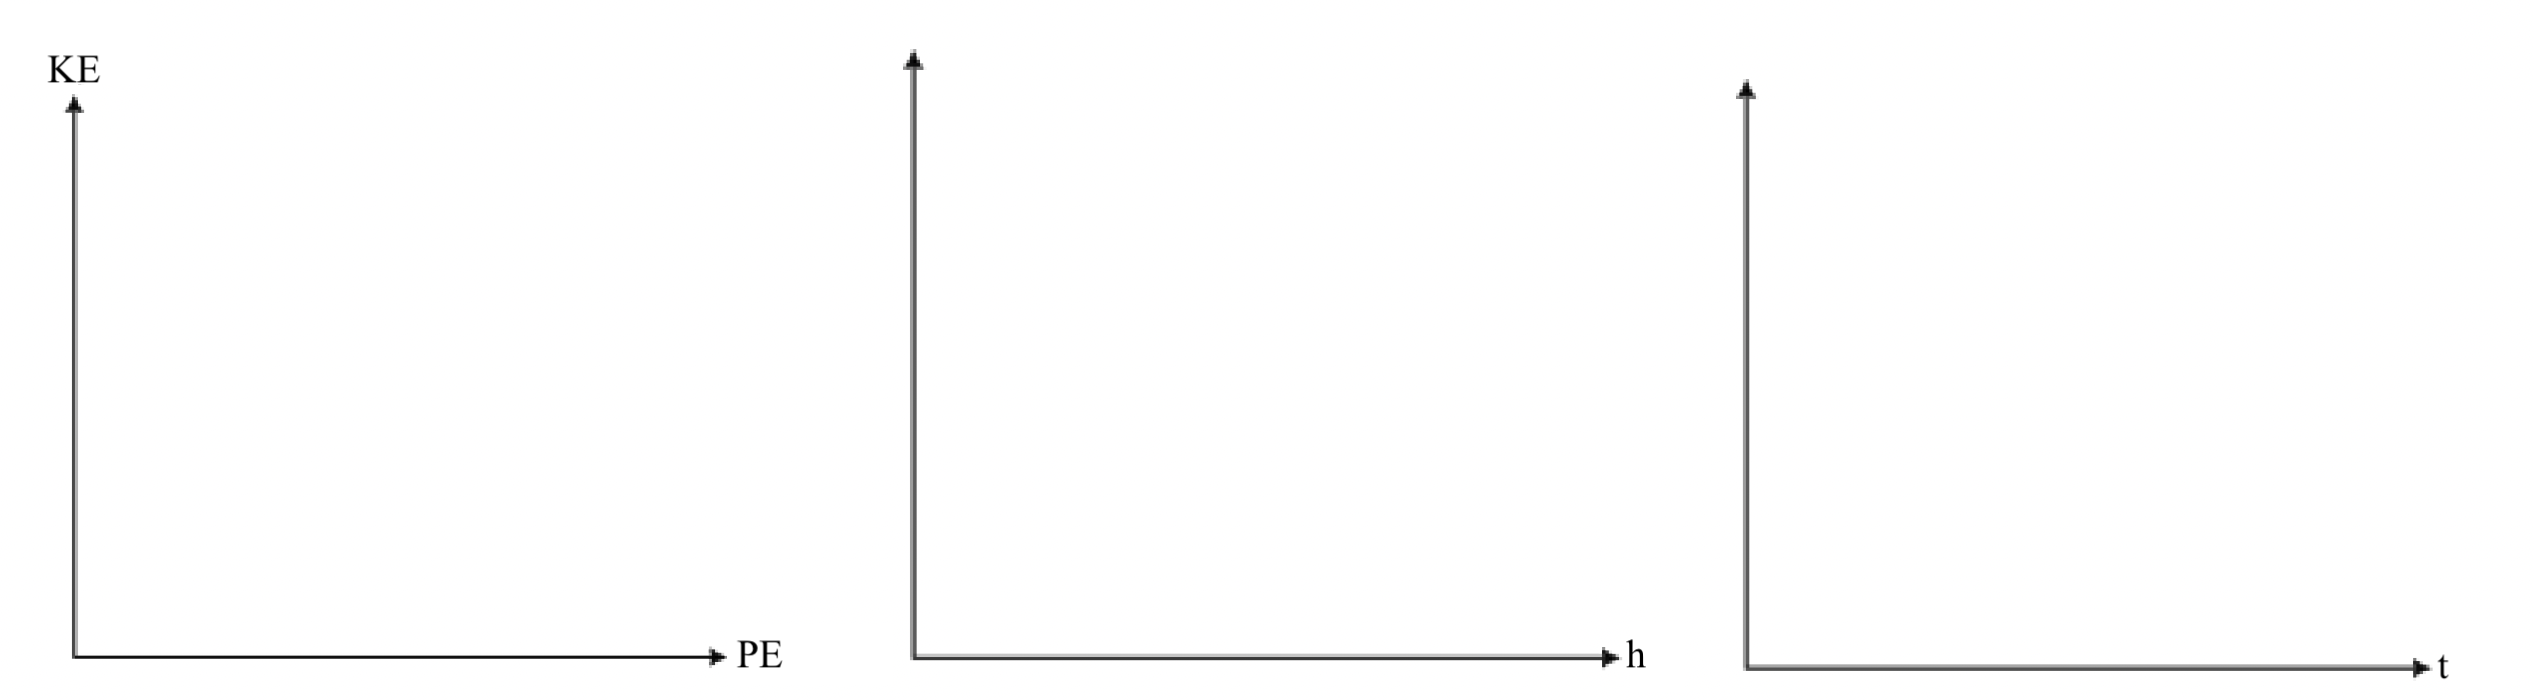
\includegraphics[width=\textwidth]{assets/4aad36d4.png}
        \par}
\end{frame}


\begin{frame}{}
    小孩推了玩具車一下,玩具車便沿粗糙斜面向上移動。作用於玩具車的摩擦力不變 下列哪一幅圖最能顯示玩具車上斜時不同能量隨玩具車移動距離的變化?\\The child pushed the toy car once, and the toy car started moving upwards along a rough incline. The frictional force acting on the toy car remains constant. Which of the following images best illustrates the variation of different energies with the distance the toy car travels uphill?
    {\par\centering
    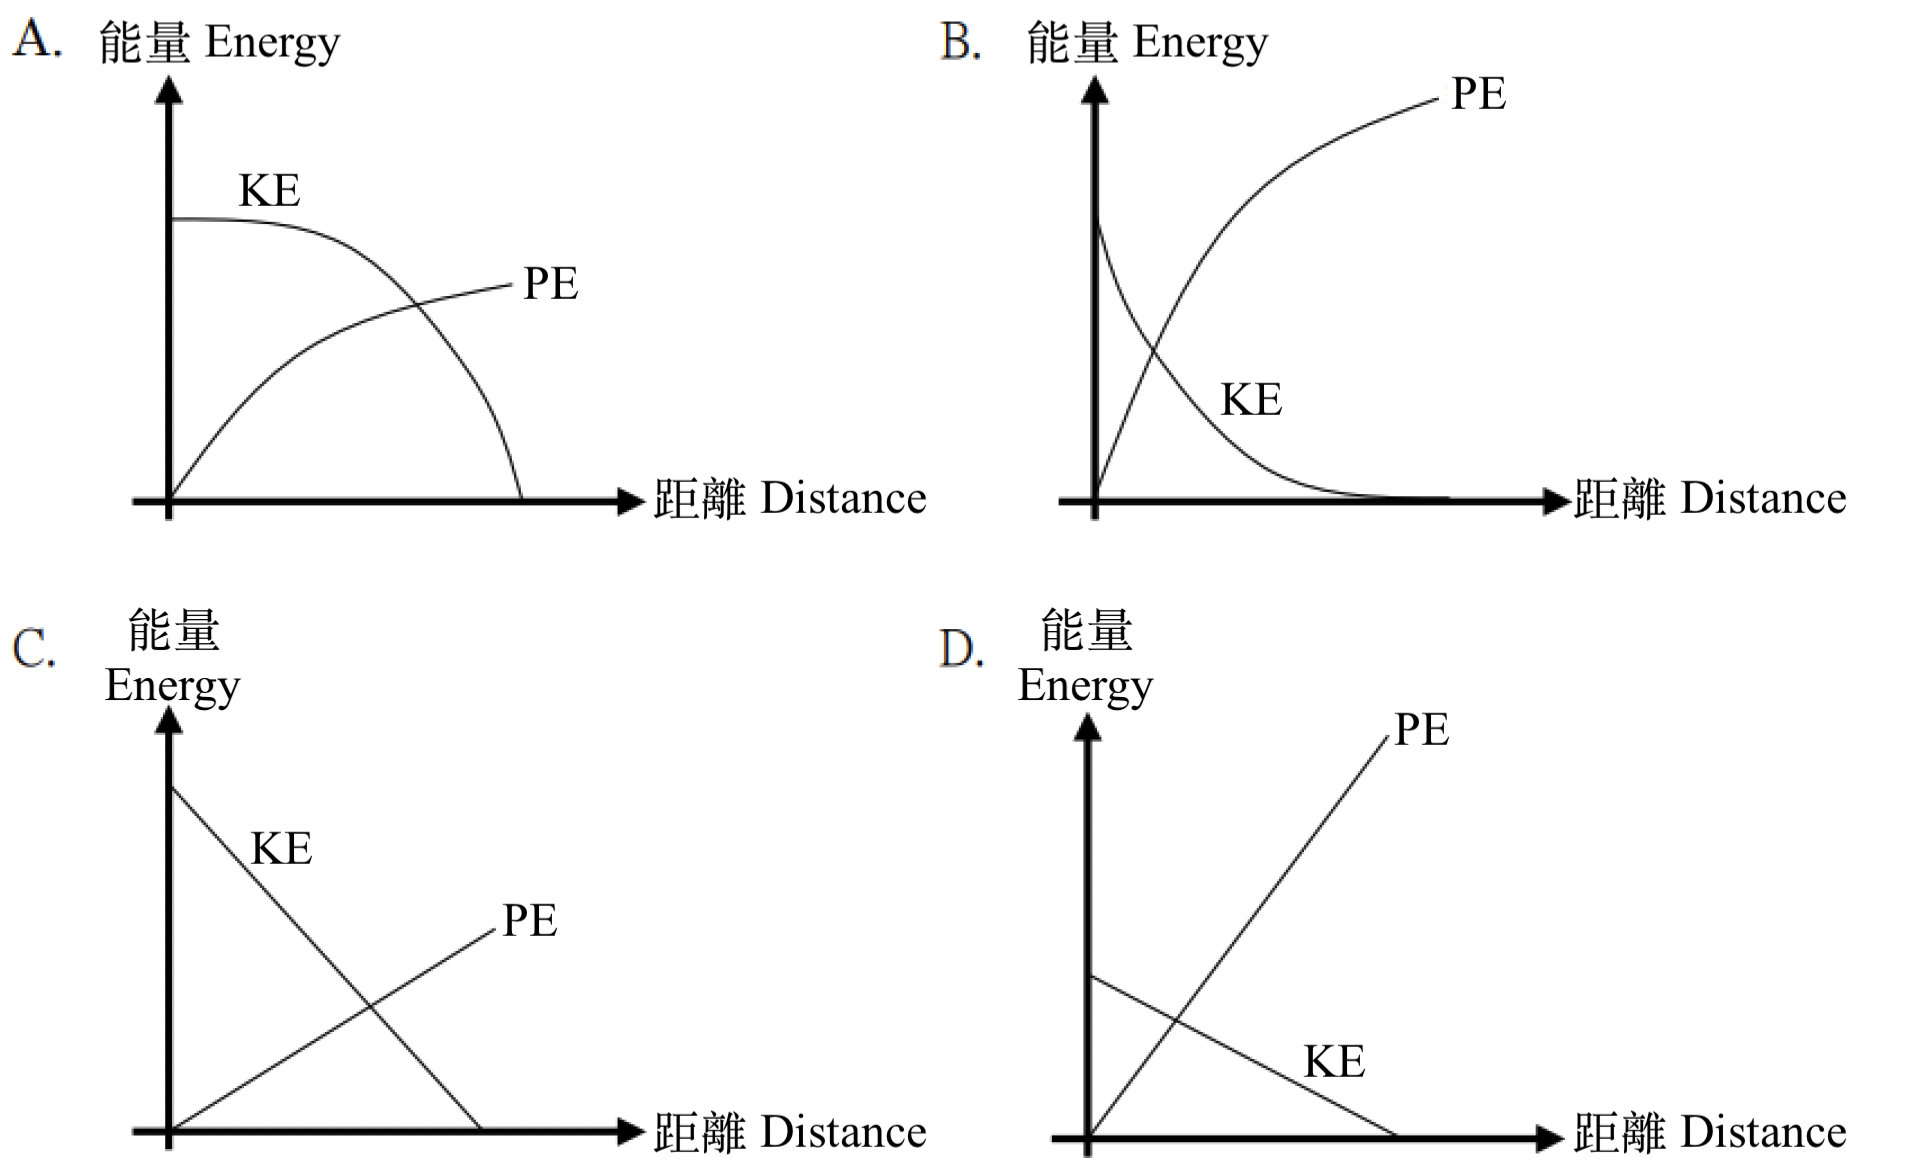
\includegraphics[width=.6\textwidth]{assets/6f1283a3.png}
    \par}
\end{frame}


\begin{frame}{}
    以下哪一個圖表最能反映物件的運動距離s與動能(KE)之間的變化?\\Which of the following best reflects relationship between KE and object distance s?
    {\par\centering
    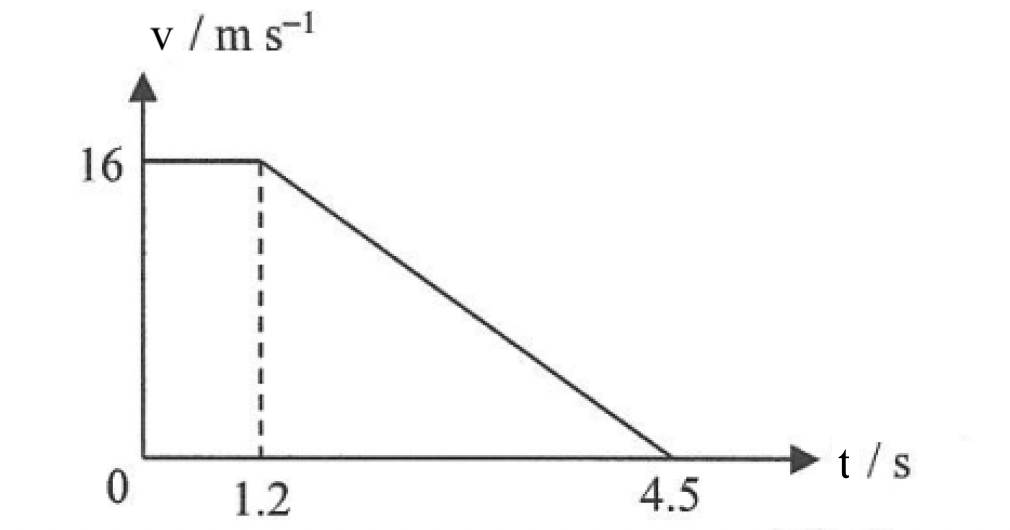
\includegraphics[width=.3\textwidth]{assets/59346db9.png}
    \par}
    {\par\centering
    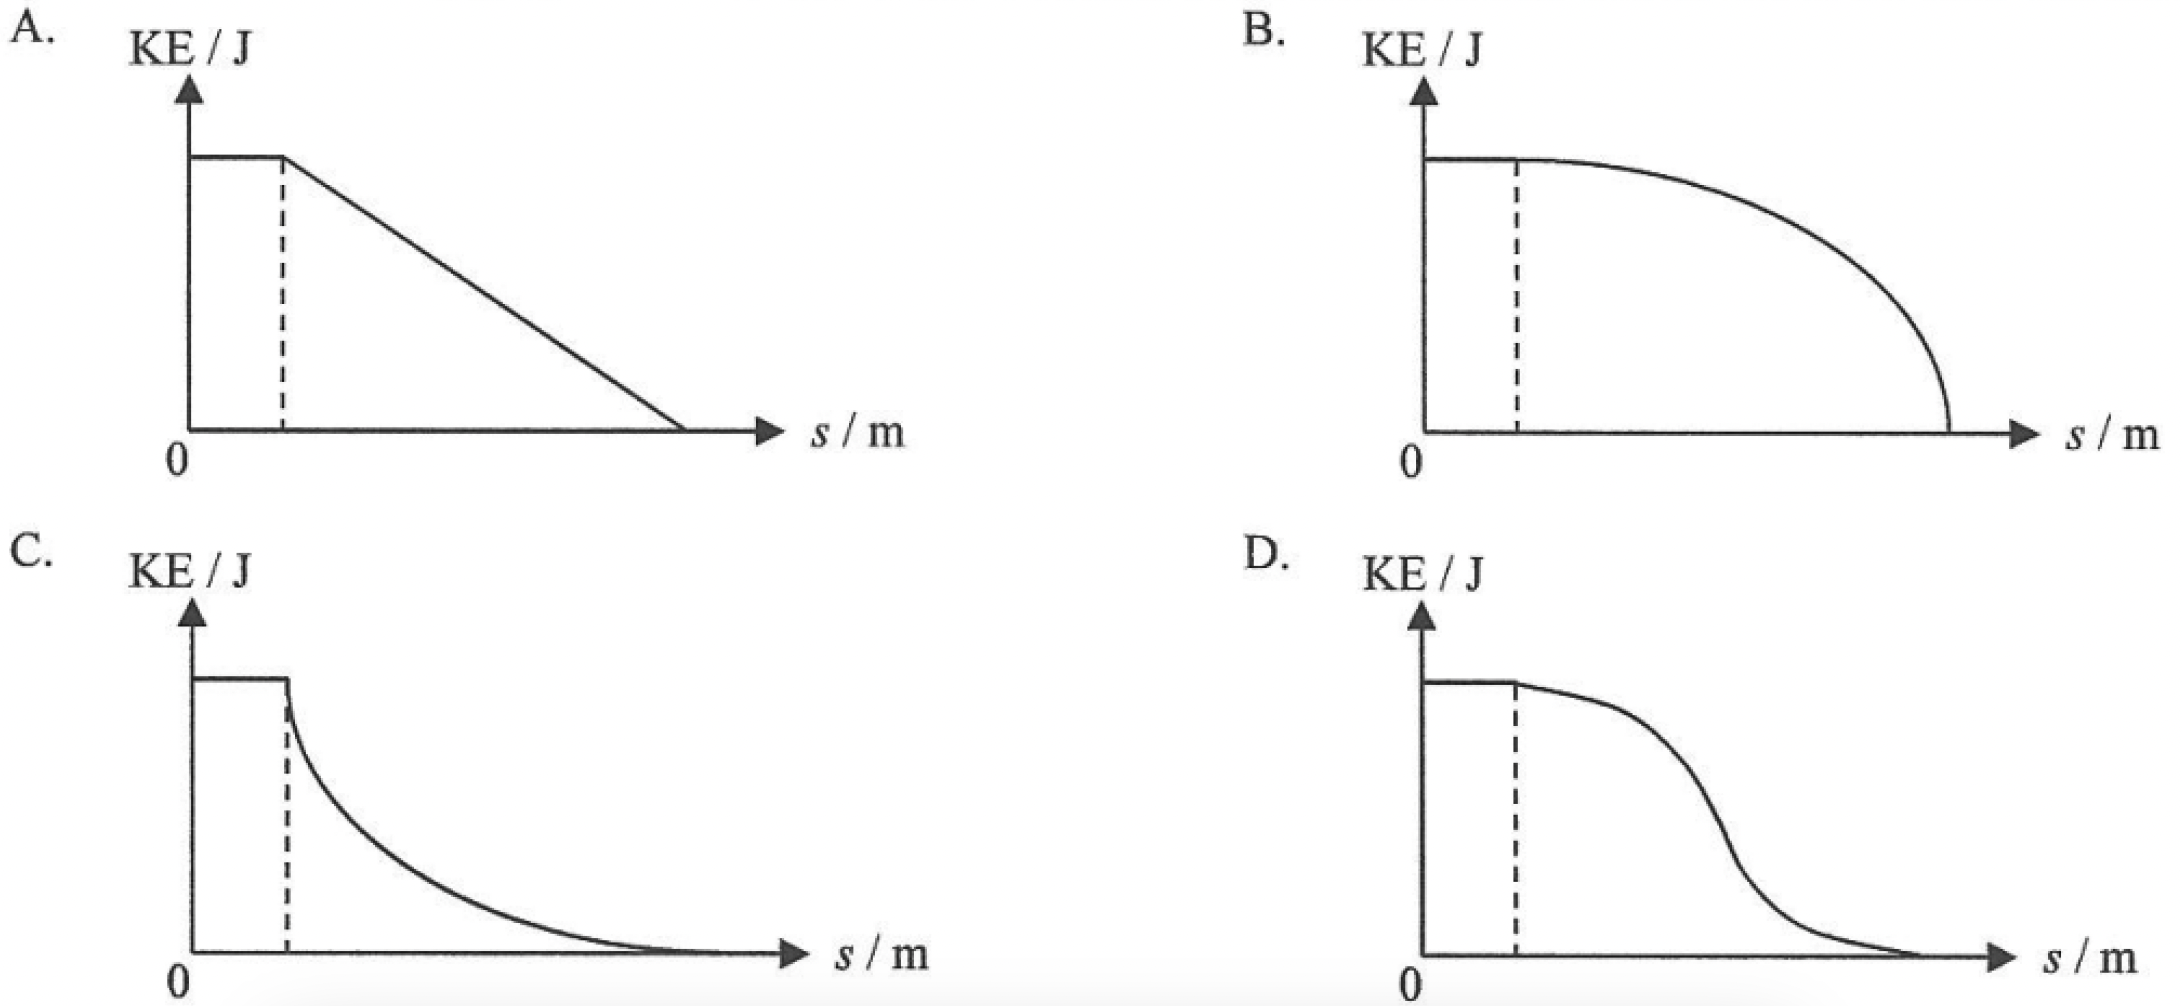
\includegraphics[width=.6\textwidth]{assets/fed589c5.png}
    \par}
\end{frame}


\begin{frame}{功率Power}
    功率是能量的轉移率,定義如下︰\\Power is the rate of transfer of energy, it is defined as follow:
    \begin{alertblock}
        {功率Power P}
        \begin{equation}
            \textrm{功率Power P}=\frac{\textrm{轉移的能量Energy transfered}}{\textrm{所需的時間Time needed}}
        \end{equation}
    \end{alertblock}
    單位Unit: [\unit{J.s^{-1}}] 或[W]
\end{frame}

% \begin{frame}{功率Power}
%     \begin{exampleblock}
%         {功率和速率的關係Relationship between power and speed}
%         \begin{align*}
%             P=F\cdot v
%         \end{align*}
%     \end{exampleblock}

% \end{frame}

\begin{frame}{功率Power}
    \begin{exampleblock}
        {功率和速率的關係Relationship between power and speed}
        \begin{align*}
            P=F\, v
        \end{align*}
    \end{exampleblock}
    如果$F$ 和 $v$ 成一個夾角 $\theta$,\\If there is included angle $\theta$ between $F$ and $v$,
    \begin{alertblock}
        {功率和速率的關係Relationship between power and speed}
        \begin{equation}
            P=F\, v\cos\theta
        \end{equation}
    \end{alertblock}
    {\par\centering
    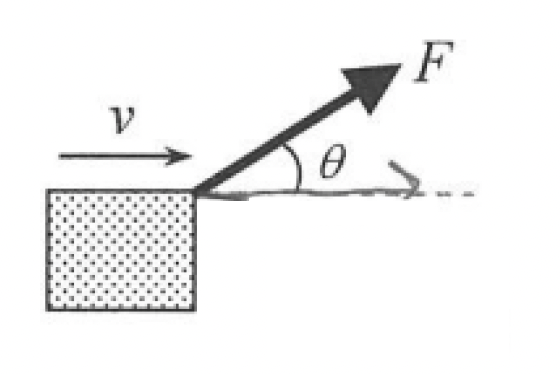
\includegraphics[width=.3\textwidth]{assets/5b4639e3.png}
    \par}
\end{frame}


\begin{frame}{功率Power}

    \begin{itemize}
        \item 假設汽車以勻速前進:\\Assuming the car is moving in constant speed:
              \begin{itemize}
                  \item 汽車的輸出功率Engine's power output $=F\, v$
                  \item 阻力導致的功率損耗Power loss by resistance  $=-f\, v$
              \end{itemize}
    \end{itemize}\bigskip
    {\par\centering
        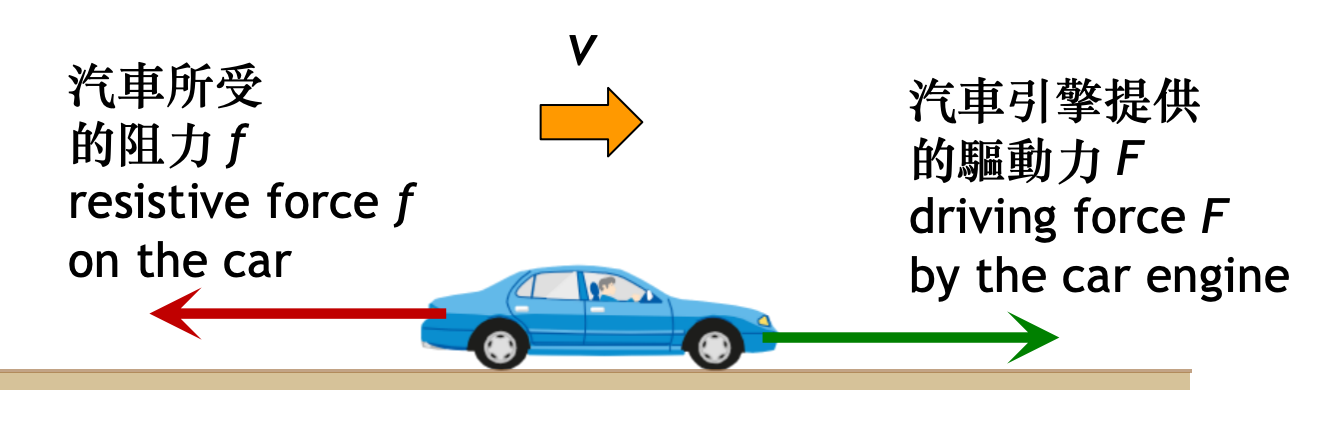
\includegraphics[width=0.66\textwidth]{assets/b805447e.png}
        \par}
\end{frame}

\begin{frame}{瞬時功率Instantaneous power}
    \begin{itemize}
        \setlength{\itemsep}{10pt}
        \item 瞬時功率Instantaneous power\\$=\textrm{(瞬時)施力(Instantaneous) Applied force}\times\textrm{瞬時速率Instantaneous speed}$
        \item 平均功率 average  power\\$=\textrm{平均施力Average applied force}\times\textrm{平均速率 average speed}$
        \item [] $=\dfrac{\textrm{總能量轉移 Total energy transfer}}{\textrm{所需時間Time needed}}$
    \end{itemize}
\end{frame}

\begin{eg}
    某人以 \vel{3} 的加速度沿傾角 \dg{25} 的斜面上升。他的質量是40 kg。忽略空氣阻力。 \\A person ascends along an inclined plane at \dg{25} above the horizontal with the acceleration \vel{3}. His mass is 40 kg. Neglect air resistance.
    \begin{itemize}
        \item [(a)] 求他在\vel{6}時的輸出功率。 \\Find his output power when his speed is \vel{6}.
    \end{itemize}
\end{eg}
\begin{eg}
    某人以 \vel{3} 的加速度沿傾角 \dg{25} 的斜面上升。他的質量是40 kg。忽略空氣阻力。 \\A person ascends along an inclined plane at \dg{25} above the horizontal with the acceleration \vel{3}. His mass is 40 kg. Neglect air resistance.
    \begin{itemize}
        \item [(b)] 若他的輸出功率不變,他的加速度會保持 \vel{3} 嗎?解釋你的答案。 \\If his power maintains unchanged, will his acceleration remains \vel{3}? Explain your answer.
    \end{itemize}
\end{eg}

\begin{frame}{效率Efficiency}
    \par
    {\par\centering
        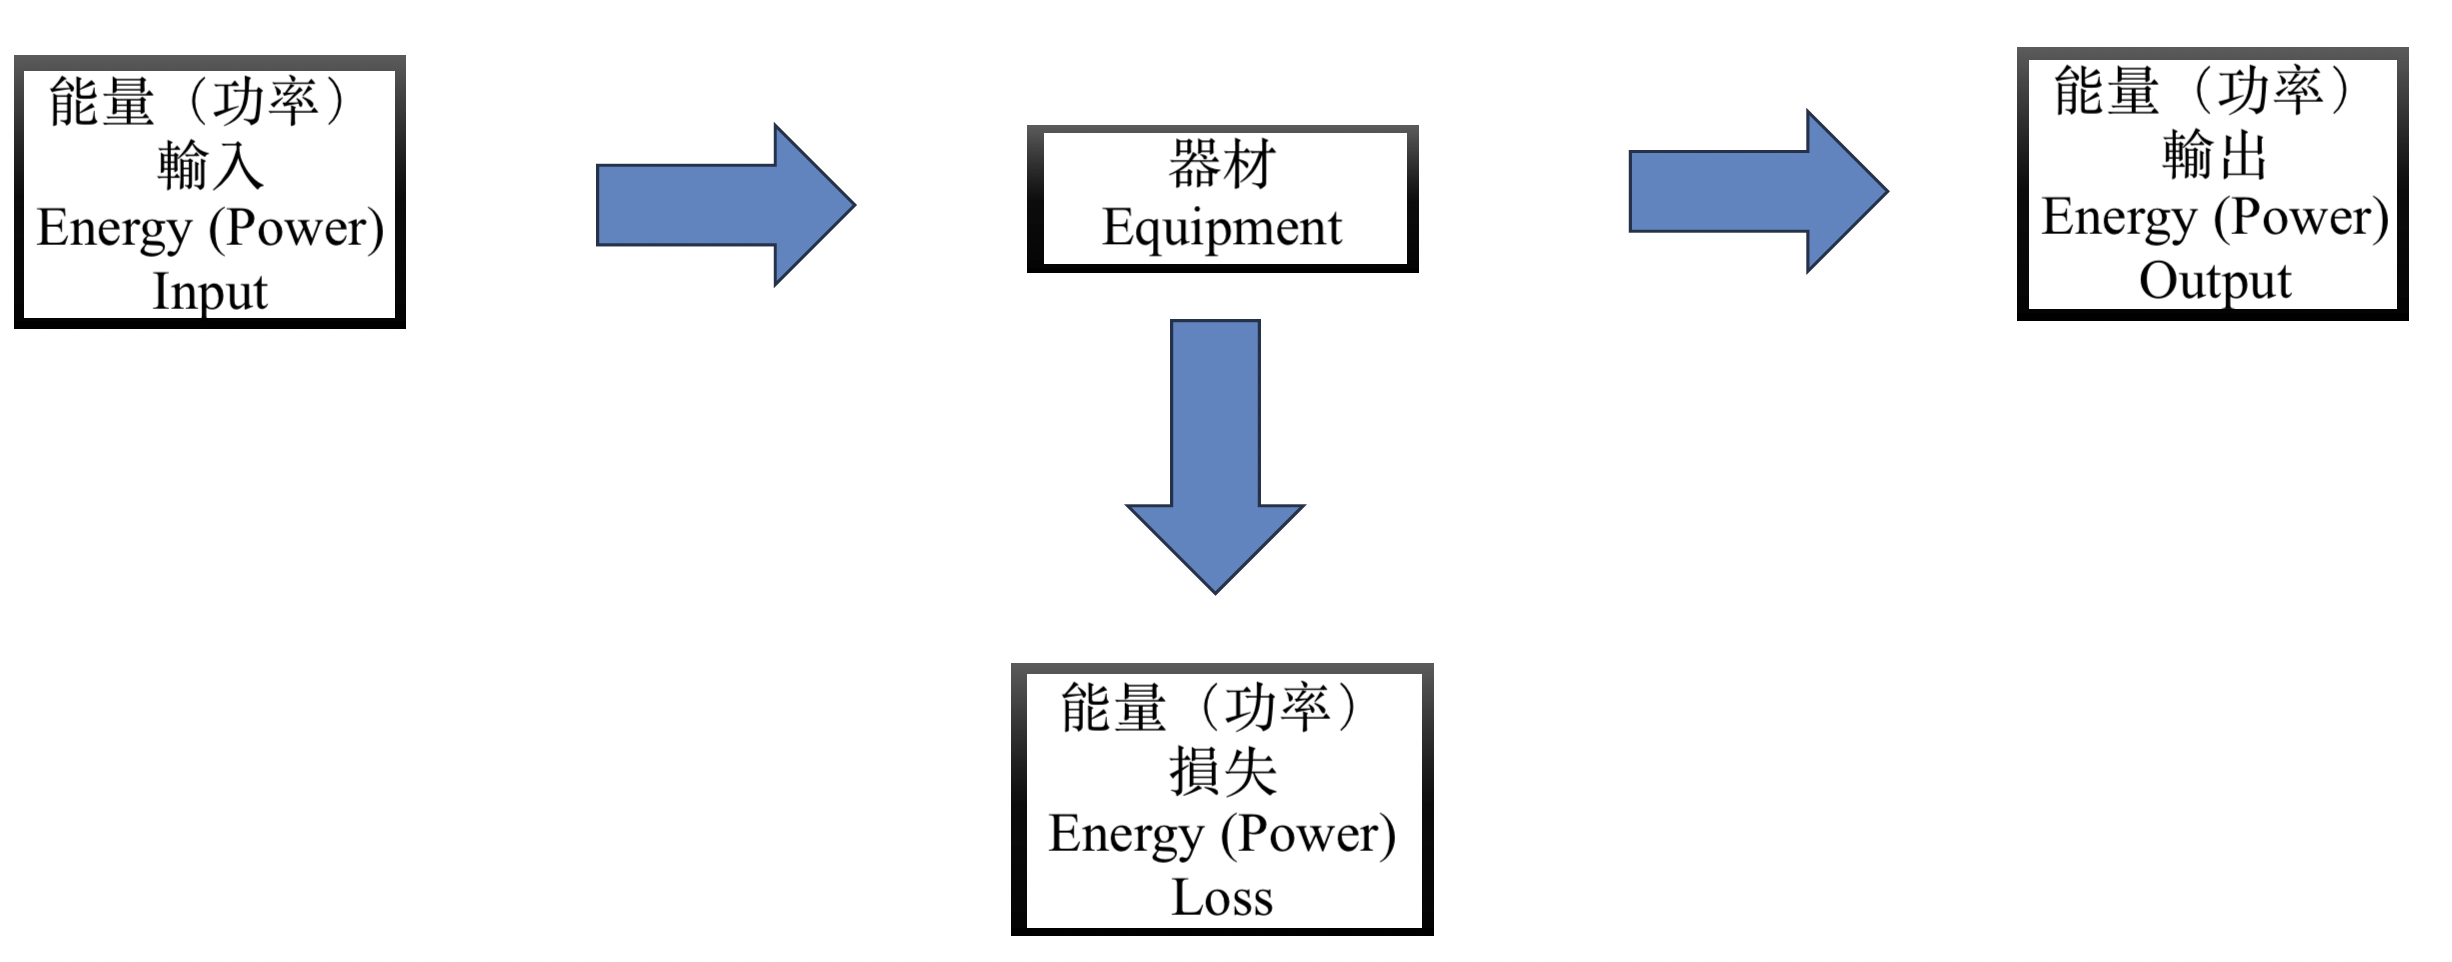
\includegraphics[width=\textwidth]{assets/119333e7.png}
        \par}

    \begin{itemize}
        \item [] $\therefore E_{In} = E_{Out} + E_{Loss}$
        \item [] $\therefore P_{In} = P_{Out} + P_{Loss}$
    \end{itemize}
\end{frame}
\begin{frame}{效率Efficiency}
    \begin{exampleblock}
        {器材的效率$\eta$ Efficiency of an equipment $\eta$}
        \begin{align*}
            \eta & = \frac{\textrm{有效的能量輸出Useful energy output}}{\textrm{總能量輸出Total energy ouput}} \\
                 & =\frac{\textrm{有效的功率輸出Useful power output}}{\textrm{總功率輸出Total power ouput}}
        \end{align*}
    \end{exampleblock}
\end{frame}

\begin{eg}
    現利用滑輪系統把一負荷提升 2 m 。輸入的能量爲5000 J 。若滑輪系統的效率 爲 80\%,求該負荷的重量。\\Using a pulley system, a load is lifted by 2 m. The input energy is 5000 J. If the efficiency of the pulley system is 80\%, determine the weight of the load.
\end{eg}

\begin{eg}
    某人利用一個和水平成 \dg{30} 的光滑科面提升一質量為 50 kg 的板 塊,如圖所示。該鈄面長 6 m。這人用了 30 s 將板塊由鈄面的底部拉至頂部。求這人的平均有效輸出功率。\\A person uses a smooth inclined plane, inclined at \dg{30}  with the horizontal, to lift a 50 kg mass block, as shown in the image. The length of the inclined plane is 6 m. It takes the person 30 s to pull the block from the bottom to the top of the inclined plane. Calculate the person's average effective output power.
        {\par\centering
            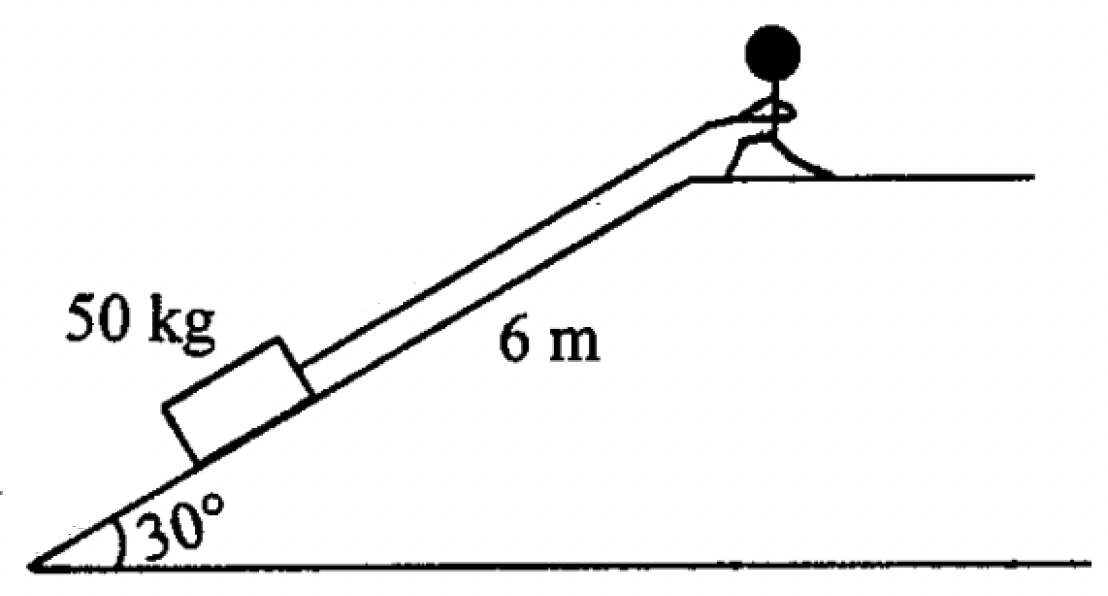
\includegraphics[width=.4\textwidth]{assets/188224a3.png}
            \par}

\end{eg}

\begin{eg}

\end{eg}

\begin{eg}
    某遊樂場內的摩天輪直徑長18m,只載有一名質量爲 60kg 的乘客,且以 勻速轉動。該乘客從輪的最低點轉至最高點需時 80s。求摩天 輪電動機的平均有效輸出功率。\\In a certain amusement park, the Ferris wheel has a diameter of 18m and carries only one passenger with a mass of 60kg. It rotates at a constant speed. It takes 80 s for the passenger to go from the lowest point to the highest point of the wheel. Calculate the average effective output power of the Ferris wheel motor.
\end{eg}











\end{document}